% !Mode:: "TeX:UTF-8"
%%==================================================
%% diss.tex for SJTU Master Thesis
%% based on CASthesis
%% modified by wei.jianwen@gmail.com
%% version: 0.3a
%% Encoding: UTF-8
%% last update: Dec 5th, 2010
%%==================================================

% 字号选项: c5size 五号(默认) cs4size 小四
% 双面打印(注意字号设置)
\documentclass[cs4size, a4paper, twoside]{sjtumaster-xetex}
\usepackage{algorithm}
\usepackage{algorithmic}



% 单面打印(注意字号设置)
% \documentclass[cs4size, a4paer, oneside, openany]{sjtumaster-xetex}


% \usepackage[sectionbib]{chapterbib}%每章都用参考文献

\newboolean{DOIT}
\setboolean{DOIT}{false}%编译某些只想自己看的内容,编译true,否则false

%% 行距缩放因子(x倍字号)
\renewcommand{\baselinestretch}{1.3}

% 设置图形文件的搜索路径
\graphicspath{{figure/}{figures/}{logo/}{logos/}{graph/}{graphs}}

%%========================================
%% 在sjtumaster-xetex.cls中定义的有用命令
%%========================================
% \cndash 中文破折号
% 数学常量
% \me 对数常数e
% \mi 虚数单位i
% \mj 虚数单位j
% \dif 直立的微分算符d为直立体。
% 可伸长的数学箭头、等号
% \myRightarrow{}{}
% \myLeftarrow{}{}
% \myBioarrow{}{}
% \myLongEqual{}{}
% 参考文献
% \upcite{} 上标引用
%%========================================


\begin{document}

%%%%%%%%%%%%%%%%%%%%%%%%%%%%%%
%% 封面
%%%%%%%%%%%%%%%%%%%%%%%%%%%%%%

% 中文封面内容(关注内容而不是形式)
\title{基于衣服属性感知的人体姿势预测}
\author{张卫鹏}
\advisor{俞勇教授}
\degree{硕士}
\defenddate{}
\school{上海交通大学}
\institute{计算机科学与工程系}
\studentnumber{1120339035}
\major{计算机应用}

% 英文封面内容(关注内容而不是表现形式)
\englishtitle{Clothing Attribute Aware Pose Estimation}
\englishauthor{\textsc{Weipeng Zhang}}
\englishadvisor{Prof. \textsc{Yong Yu}}
\englishschool{Shanghai Jiao Tong University}
\englishinstitute{\textsc{Depart of Computer Science and Engineering} \\
  \textsc{Shanghai Jiao Tong University} \\
  \textsc{Shanghai, P.R.China}}
\englishdegree{Master}
\englishmajor{Computer Science}
\englishdate{}

% 封面
\maketitle

% 英文封面
\makeenglishtitle

% 论文原创性声明和使用授权

\makeDeclareOriginal
\makeDeclareAuthorization

%%%%%%%%%%%%%%%%%%%%%%%%%%%%%%
%% 前言
%%%%%%%%%%%%%%%%%%%%%%%%%%%%%%
\frontmatter

% 摘要
% !Mode:: "TeX:UTF-8"
%%==================================================
%% abstract.tex for SJTU Master Thesis
%% based on CASthesis
%% modified by wei.jianwen@gmail.com
%% version: 0.3a
%% Encoding: UTF-8
%% last update: Dec 5th, 2010
%%==================================================

\begin{abstract}
近年来在图像分析、动作识别等领域,人体姿势预测这个基本问题得到了科学家们广泛的关注.
从已有的工作来看,人的头部、身躯等部位已经取得了很高的精度,但是手臂由于其丰富的姿势变化,目前还只有0.7的精度,这几乎是人体姿势预测领域最大的挑战。
一个明显的想法是,衣服属性信息对于姿势的精准预测是有很大的帮助.
前人也有很多利用衣服属性信息去帮助姿势预测的工作,但是需要人为的去标注大量的衣服属性标签,这是一项极其耗时的工作。

在本文中,我们提出了基于隐式衣服属性的人体姿势预测。
我们通过对图画式结构进行扩展来形式化人体姿势预测问题,特别地,我们将衣服属性作为隐变量来建模。
跟传统的基于标注信息进行预测的方法不同,我们不需要显示的标注额外的信息,而且可以高效的进行求解。
在本文中,我们定义了几种比较重要的衣服属性,并且建立了衣服属性和人体部位之间的关系(比如袖子和手臂等)。
进而,我们设计了两种特征,一是人体躯干对应的特征,二是人体躯干和衣服属性的联合特征。
我们采用隐式结构式支持向量机算法来进行模型的训练。
所有的隐变量问题都会涉及到隐变量的初始化问题,我们采用K-Means聚类算法来初始化隐变量。
接着,我们采用增量迭代的方式来进行参数的学习,即就是最小化隐式结构式支持向量机的目标函数。
更为详尽的,我们采用迭代的方式来训练模型,首先当衣服属性变量确定的时候,我们采用动态规划的算法进行人体姿势的求解。
另一步是,当人体姿势确定的时候,我们可以采用第三章提出的算法来确定衣服属性的变量。
在两个公开的数据集上,我们进行了有力的实验,结果显示我们的方法超过了传统最好的方法,
特别是在手臂的预测上,我们比前人工作提高了8个百分点,并且我们将具有同样衣服属性的照片聚在了一起。

\keywords{\large 姿势预测 \quad 结构式学习 \quad 隐变量}
\end{abstract}

\begin{englishabstract}
As a fundamental technique with wide applications in image parsing, action recognition, etc.,
human pose estimation (HPE) has been extensively investigated in recent years.
For accurate and reliable estimation of the human pose, it is well-recognized that the clothing attributes are useful and should be utilized properly.
Most previous approaches, however, require to manually annotate the clothing attributes and are therefore time-consuming.

In this paper, we shall introduce a \emph{latent} clothing attribute approach for HPE. Our approach formulates the HPE problem by extending the pictorial structure framework~\cite{ps1,ps2} and, in particular, models the clothing attributes as \emph{latent variables}. Comparing to the previous approaches that rely on label information, our latent approach, in sharp contrast, requires no explicit labels of the clothing attributes and can therefore be executed in an efficient way. We define some clothing attributes and build their connections with human parts (e.g., sleeve with arms). Some domain specific features, including \emph{pose-specific} features and \emph{pose-attribute} features, are designed to describe the connections. We utilize the latent structured support vector machines (LSSVM) for the training procedure, where the attribute values are initialized by a simple K-Means clustering algorithm. Then the model parameters are learnt by employing a relabel strategy, which minimizes the objective function of LSSVM in an ``alternating direction'' manner. More precisely, we perform an iterative scheme to train the model: Given the (latent) clothing attributes, we perform a dynamic programming algorithm to find a suboptimal solution for human pose; Given the human pose, we seek the optimal attribute values by performing a greedy search on the attribute space. We empirically show that our approach can achieve the state-of-the-art performance on two benchmarks, especially on the estimation of arms, we get the 8\% improvement than previous approaches.

\englishkeywords{\large pose estimation, structure learning, latent variables}
\end{englishabstract}


% 目录
\tableofcontents
% 表格索引
\listoftables
% 插图索引
\listoffigures

\addcontentsline{toc}{chapter}{\listfigurename} %将表格索引加入全文目录
\addcontentsline{toc}{chapter}{\listtablename}  %将图索引加入全文目录

% 主要符号、缩略词对照表
%\include{body/symbol}

%%%%%%%%%%%%%%%%%%%%%%%%%%%%%%
%% 正文
%%%%%%%%%%%%%%%%%%%%%%%%%%%%%%
\mainmatter

% symbols
\newcommand{\mU}{{\mathbf{U}}}
\newcommand{\mV}{{\mathbf{V}}}
\newcommand{\mP}{{\mathbf{P}}}
\newcommand{\mQ}{{\mathbf{Q}}}
\newcommand{\mY}{{\mathbf{Y}}}
\newcommand{\mX}{{\mathbf{X}}}
\newcommand{\vx}{{\mathbf{x}}}
\newcommand{\rR}{{\mathbb{R}}}
\newcommand{\sF}{{\mathcal{F}}}
\newcommand{\trs}{{T}}
\newcommand{\gbmf}{GFMF}
\newcommand{\cC}{C}

\newcommand{\loss}{{\mathcal{L}}}
\newcommand{\sloss}{{\mathcal{C}}}
\newcommand{\sset}{{\mathcal{S}}}
\newcommand{\vset}{{\mathcal{V}}}
\newcommand{\vp}{{\mathbf{p}}}
\newcommand{\vv}{{\mathbf{v}}}
\newcommand{\vq}{{\mathbf{q}}}
\newcommand{\vy}{{\mathbf{y}}}
\newcommand{\norm}[1]{\Vert#1\Vert}
\newcommand{\ve}{{\mathbf{e}}}
\newcommand{\vbeta}{{\mathbf{\beta}}}
\newcommand{\set}[1]{\{#1\}}
\newcommand{\abs}[1]{|#1|}


%% 各章正文内容
% !Mode:: "TeX:UTF-8"
%%==========================
%% chapter01.tex for SJTU Master Thesis
%% based on CASthesis
%% modified by wei.jianwen@gmail.com
%% version: 0.3a
%% Encoding: UTF-8
%% last update: Dec 5th, 2010
%%==================================================

%\bibliographystyle{sjtu2} %[此处用于每章都生产参考文献]
\chapter{引言}
\label{chap:intro}

\section{背景和意义}
人体工程学是计算机视觉领域的核心内容,它可以影响到人们方方面面的生活。
例如人脸识别在安全领域的应用,衣服属性分析在衣服搜索领域的应用等等。
这些技术中最基础之一是人体姿势预测。
一般来说,人体姿势预测(HPE)可以应用到很多领域,比如动作识别、图像分割等等。
然而它是一个非常困难的问题,特别是在没有任何辅助信息的情况下,而且对于手臂和腿部等变化比较丰富的人体部位。

众所周知,可以用上下文信息(比如衣服属性、边缘信息等)来解决这个难题。
在图1中,a,b,c是三个候选结果,很明显如果我们知道一些上下文信息,很容易判断出只有c是正确解。
因此,这种方法叫做上下文模型,即就是将图片上已知的信息加入到HPE问题中,来提高模型的准确性。
近来年,有很多学者做了这方面的工作\cite{deeppose,cvpr09}, 比如\cite{deeppose},他将前背景和后背景对比信息加入到人体姿势预测中。
Ladicky\cite{cvpr09}等人将人体姿势预测与图像分割联系起来,用通过这种联合学习的方式提高HPE的精度。
在Jie Shen\cite{shen2014unified}等人的工作中,他们将人体姿势和衣服属性联合起来进行求解\cite{cvpr09}。

\section{研究内容和方法}
虽然已有的很多工作利用上下文信息提高了人体姿势预测的精度,但是他们都需要进行大量的上下文信息标注才能进行训练,这个非常耗时而且不太实际,对于大数据来说。
在本文中,我们提出了基于隐式衣服属性的人体姿势预测。
我们通过对图画式结构进行扩展来形式化人体姿势预测问题,特别地,我们将衣服属性作为隐变量来建模。
跟传统的基于标注信息进行预测的方法不同,我们不需要显示的标注额外的信息,而且可以高效的进行求解。
在本文中,我们定义了几种比较重要的衣服属性,并且建立了衣服属性和人体部位之间的关系(比如袖子和手臂等)。
进而,我们设计了两种特征,一是人体躯干对应的特征,二是人体躯干和衣服属性的联合特征。
我们采用隐式结构式支持向量机算法来进行模型的训练。
所有的隐变量问题都会涉及到隐变量的初始化问题,我们采用K-Means聚类算法来初始化隐变量。
接着,我们采用增量迭代的方式来进行参数的学习,即就是最小化隐式结构式支持向量机的目标函数。
更为详尽的,我们采用迭代的方式来训练模型,首先当衣服属性变量确定的时候,我们采用动态规划的算法进行人体姿势的求解。
另一步是,当人体姿势确定的时候,我们可以采用第三章提出的算法来确定衣服属性的变量。
在两个公开的数据集上,我们进行了有力的实验,结果显示我们的方法超过了传统最好的方法,并且我们将具有同样衣服属性的照片聚在了一起。

\section{本文的贡献}
总体来说,本文有三大主要贡献:

(1)\textbf{我们提出了一个隐式衣服属性的方法,可以隐性的将衣服属性加入到人体姿势预测问题中。}
通过上述讨论可知,姿势估计和衣服属性识别这两个问题之间有很强的关联性,但是之前的工作,
无论是直接利用姿势估计来进行服饰分析,还是迭代地分割服饰再优化姿势,
或是定义一些能量函数然后通过参数来平衡姿势和服饰的权重,都没有很好地在一个框架下对这两个问题进行统一的建模求解。
在我们的工作中,考虑衣服属性的作用,并且将它作为一个隐式变量,这样就不用手动的去标注衣服属性。

(2)\textbf{我们定义了一些有效的特征来描述人体部位和衣服属性之间的关系。}
特征是用来刻画问题输入对象的重要参数,所以特征的设计选择直接影响着后续的问题建模与求解。 特征设计是机器学习领域非常重要的问题之一,往往一个问题的特征设计好坏与否直接关系到问题求解的优劣。
在我们工作中,人体肢干相关的特征,我们主要考虑两个方面,一是肢干本身的特征,二是相邻肢干的联合特征。 HOG特征在前人的很多工作中得到应用,它被证明可以很好的描述物体的形状,因而在我们的工作中,肢干本身的特征采用HOG特征。 关于相邻肢干的联合特征,我们主要考虑两个肢干的相对位置、相对角度和相对距离。


(3)\textbf{我们提出了一个高效的算法来解决有环图的预测问题(这是一个极其有难度的问题)。}
在以往的工作中,大家对于分别求解两个问题时,都假定问题满足树结构,这样可以使得求解非常高效。 但是现在我们对于两个问题同时建模,破坏了树结构的假设,为此,我们提出了一种迭代求解的算法, 在每一次的迭代过程中,人体的姿势或者衣服的属性都是固定的,从而问题可以规约成一个树模型的求解过程, 使得每一轮的求解可以使用动态规划法进行高效的求解。

\begin{figure}[tbp]
    \centering
    \subfigure[]{
        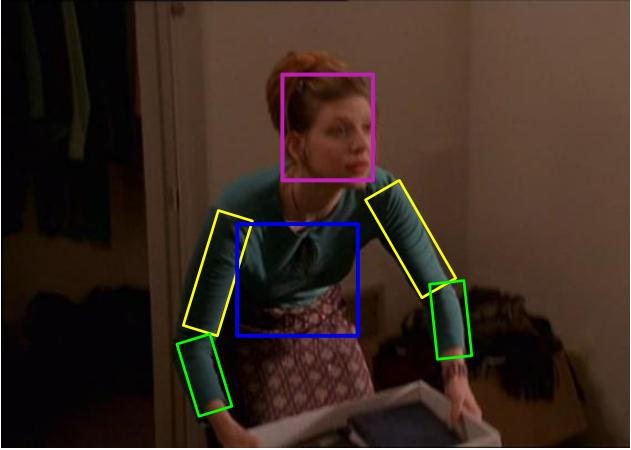
\includegraphics[width=.3\textwidth]{img/eg_a.pdf}
    }
    \subfigure[]{
        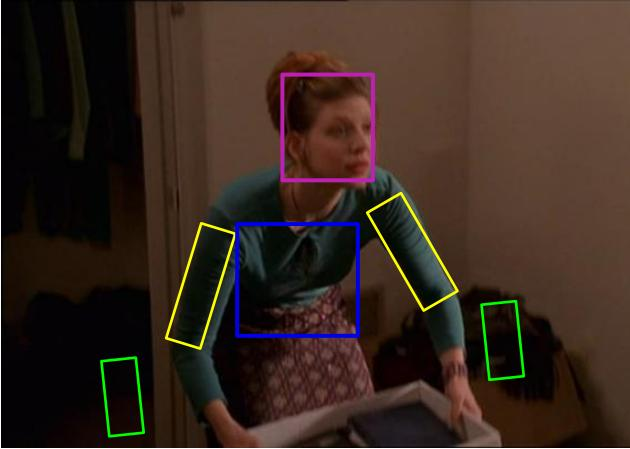
\includegraphics[width=.3\textwidth]{img/eg_b.pdf}
    }
    \subfigure[]{
        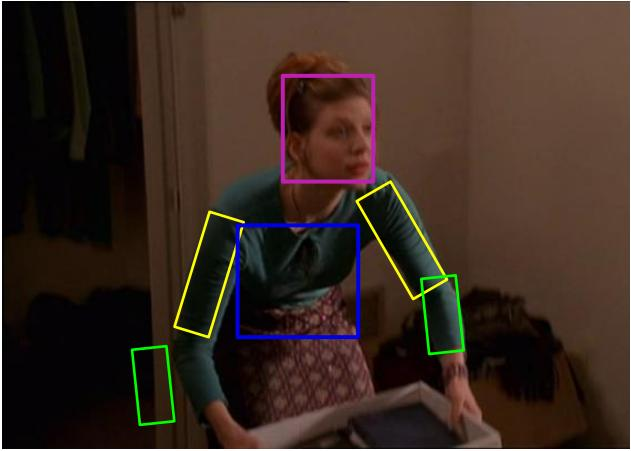
\includegraphics[width=.3\textwidth]{img/eg_c.pdf}
    }
    \caption{
    \textbf{在人体姿势预测问题中加入衣服属性的动机}
图中所示的三个人体姿势预测的结果,图(b)和图(c)中除了下臂预测错误,其它躯干预测的结果都是正确的。
对于图(c)来说,我们可以通过形状特征来得出左右手臂的不同之处,从而可以将(c)排除掉,
但是在图(b)中,左右手臂的不同之处很微小,我们很难用形状特征来区分出左右手臂。
如果我们知道图中衣服属性的类别值,比如袖子的类别和颜色等。
这样我们就可以根据袖子的颜色或者类别值来区分左右手臂,因为图(b)中左右手臂对应的衣服属性袖子颜色不一致。
最后,我们得到了正确的预测结果,即图(a)。
    }
    \label{fig:eg}
\end{figure}


\section{论文组织}
接下来我们将逐章来介绍我们的工作。
在第二章中,我们介绍了相关的工作,主要分为人体姿势预测(Human Pose Estimation)、衣服属性分析(Clothing Attribute Analysis)、隐变量结构式学习(Structure Learning with Latent Variables)等特定问题领域来介绍。
在第三章中,我们会介绍本文工作的问题背景,主要对本文中涉及到的技术做一个很好的概括。
主要分为图模型(Graphic Model)、图画式结构(Pictorial Structure)、结构式学习(Structure Learning)、形变部位模型(Deformable Part Model)等知识领域来介绍。
在第四章中,我们主要介绍了我们提出的模型和算法,主要分为联合特征设计、模型训练、姿势预测算法等部分来介绍。
第五章我们节选了部分之前跟人体姿势相关的工作来讲述,主要包括基于多媒体数据的事件挖掘(Event Detection)、基于电商平台的衣服搜索(Clothing Search)、基于图片的广告推荐(Advertisement Recommendation)等。
主要阐述人体姿势预测在这些问题上的应用。
在第六章中,我们介绍了实验部分,对数据集、评测指标、实验结果等进行了详细的介绍。
第七章,我们进行了总结,并对未来的工作进行了展望。

\section{本章小结}
本章中,我们简要的介绍了前人在人体姿势识别方面的工作,以及他们的不足,从而提出我们的方法,
克服前人工作的不足支持。
并且我们通过例子说明了加入衣服属性的良好效果。


% !Mode:: "TeX:UTF-8"
%%==========================
%% chapter01.tex for SJTU Master Thesis
%% based on CASthesis
%% modified by wei.jianwen@gmail.com
%% version: 0.3a
%% Encoding: UTF-8
%% last update: Dec 5th, 2010
%%==================================================

%\bibliographystyle{sjtu2} %[此处用于每章都生产参考文献]
\chapter{相关工作}
\label{chap:related}
就像之前说过的那样,人体姿势预测是一个很难的问题,特别是在没有上下文约束信息的情况下。
有一些研究者做了一些在三维(3D)空间去解决人体姿势识别问题的工作\cite{burenius20133d,ics14cvpr}。
在工作\cite{burenius20133d}中,他们将二维(2D)空间图画式框架算法\cite{ps1,ps2}扩展到了三维(3D)空间,并且提出了一个新的框架来对姿势位置、相邻躯干角度等。
Shotton等人在工作\cite{shotton2013real}中,提出了一个实时的算法去估计三维(3D)空间的人体姿势,
这是可以用在工业界的算法,因为实时性可以保证我们做出产品级的姿势识别程序。

\section{人体姿势预测}
大部分的人体姿势识别的工作都是基于二维(2D)空间的图片为数据基础,在这些工作中,他们用带方向的模板方块去表示一个人体躯干,
各个方块之间是独立分开的,这可以提供一个比较简单的方式来描述人体躯干之间的结构。
显而易见,这种方式对于很多比较复杂的姿势是无法处理的\cite{nips06,cvpr10},比如有些躯干是被遮挡的,没有直接显现在图片中。
对于这种复杂的情况,在论文\cite{deva11}中,一种更高级的方式被提出来描述带方向的人体躯干,他们用多个带方向的模板来描述每一个人体躯干,
每一个带方向的模板被设定有一个属性“类别”。有趣的是,这个新的模型可以通过调整弹簧结构中相邻节点的关系而模拟这种躯干被遮挡的情况。

还有一些工作希望通过一些相关技术来增强人体姿势预测的精确度,比如图像分割技术等。
在论文\cite{eccv10}中,一堆图像特征(比如边缘反馈和区域分割)被结合进来增强人体姿势预测的精度。
在论文\cite{songchun}中,图像背景被描述为遵循高斯分布,通过高斯模型去获得更多的图像信息。
在论文\cite{mixing}中,他们采用了一种两步近似算法来提高视频中人体躯干中下臂的预测精度,这种算法的输出结果要求每一种解都跟周边有比较高的对比度。

在特征上,传统方法一般都是采用方向梯度算子(HOG)这类形状特征来进行特征的设计,
但是一些反应外观的特征(比如颜色、纹理特征等)对于人体姿势预测也是很有帮助的\cite{bmvc09}。
一般而言,这些反应外观的特征都是描述衣服的特征,因为数据集中人一般都是穿衣服的,而这些外观特征恰好描述了衣服属性。
通过图\ref{fig:eg}易知,人体躯干和衣服属性之间有很强的联系。
一些衣服属性识别的工作\cite{clotheccv,clothliu,poselets,junchi},他们首先进行人体姿势预测的算法,然后利用人体姿势预测的结果来作为衣服属性识别算法的输入,
由于有了人体姿势预测的结果,所以可以很容易的提取出人体躯干对应的衣服属性,从而进行衣服属性分析识别。
但是很明显,这种方法严重依赖于人体姿势预测的结果。
还有一些方法\cite{cloth12,shen2014unified},他们观察到不仅人体姿势预测的结果可以帮助到衣服属性的识别,而且衣服属性的识别也可以帮助提高人体姿势预测的精度。
所以这些方法将人体姿势预测问题和衣服属性识别问题联合起来,将两者的约束关系利用进来,同时提高人体姿势预测和衣服属性识别的精度。
然而,人体姿势预测问题的标准数据集一般都是只有人体躯干的标签信息,没有提供额外的衣服属性标签信息,所以这些方法都需要进行大量的衣服属性标注工作,
这无疑是非常耗时的一项工作。在我们的工作中,我们会将衣服属性作为隐变量加入到人体姿势预测问题中,所以避免了大量的、耗时的标注工作。

\section{衣服属性分析}
衣服属性分析也是计算机视觉领域中一个极其重要的问题,而且衣服属性分析的结果可以直接应用到电商领域。
还有很多其它工作也将衣服属性分析结合进各自的模型中,来提高精度。
在论文\cite{clothrec}中,Liu等人希望针对特定的场景来推荐合适的衣服。为了解决这个问题,首先需要建立一个模型来刻画图像底层特征和衣服推荐场景的关系,
他们提出了一个算法框架,先识别出衣服属性,然后通过衣服属性的语义信息来推荐匹配的衣服。
在论文\cite{action}中,跟本文类似的衣服属性技术被用到动作识别当中。
但是,有个关键的区别:论文\cite{action}中的衣服属性是被用作一个中间过程的结果,然后更高层的任务来采用衣服属性的结果去完成。
而在我们的工作中,衣服属性是跟人体躯干结合在一起的,构建一个联合模型来求解我们的问题。
我们提出的模型采用重标记的方法来同时优化人体躯干变量和衣服属性变量。

\section{隐变量结构式学习}
% ICML09_LatentSSVM
很多前人的工作都致力于将隐变量加入到判别式模型中,来通过加入隐变量的方式提高模型的预测精度。
这种想法来自于计算机视觉领域,在物体识别领域,一个很自然的想法是将人体躯干或者物体当作隐变量去建模。
论文\cite{HCRF}提出了隐式随机条件场,它是一种针对结构式预测的包含隐变量的判别式概率模型,
并且展示了该算法在两个计算机视觉领域的任务。
在自然语言理解领域,也有一些工作\cite{dlglv}来应用这种包含隐变量的判别式概率模型,
例如用这种判别式的方式来加入隐式的标注信息,来进行PCFG的训练。
由于加入了隐变量,所以一般结构式学习就会变为非凸问题,
所以一般采用基于梯度的方法来优化这种问题的非凸似然函数。

我们工作中采用的Concave-Convex(凹-凸)过程\cite{CCP}是最小化非凸函数的一般解决方案,这跟一般的非凸函数优化问题是一个类问题。
最近几年,出现了不少的应用来采用这个算法去解决实际问题,
包括去训练非凸的SVM(支持向量机)和直推式SVM(支持向量机)\cite{tcs}。
论文\cite{Vishwanathan05kernelmethods}中提高的方法,用CCCP去处理SVM和Gaussian Processes(高斯过程)中的缺失数据。
而类似的一篇文章\cite{llsvm}是非概率的模型,并避免了分割函数的计算,这对于结构式预测是非常关键的。
近年来,CCCP也被用来解决结构式预测中损失边界比较紧密的非凸问题\cite{boundSE}。

在计算机视觉领域,近年来有很多工作在用max-margin(最大化间隔)的规则去训练隐式随机条件场模型\cite{muldpm,maxHCRF}。
但是这些工作都是专注在分类问题上,只能说是结构式学习的特例而已。
论文\cite{muldpm}提出了一个最大化间隔形式和算法来进行结构化结果预测,并且可以使用隐变量。
这也是隐变量结构式学习领域中最经典的一篇工作。


\section{本章小结}
本章介绍了三个方面的相关工作,包括人体姿势预测、衣服属性分析和隐变量结构式学习。
可以看出人体姿势预测问题和衣服属性分析问题有着极其密切的联系,
二者其一都对另一个问题有极其大的帮助,所以我们通过建立关于两个问题的联合特征来提高人体姿势预测的精度。
由于标准数据集对衣服属性标签信息的缺失,我们自然而然想到了把衣服属性作为隐变量,
利用隐变量结构式学习去解这个问题。


% !Mode:: "TeX:UTF-8"
%%==========================
%% chapter01.tex for SJTU Master Thesis
%% based on CASthesis
%% modified by wei.jianwen@gmail.com
%% version: 0.3a
%% Encoding: UTF-8
%% last update: Dec 5th, 2010
%%==================================================

%\bibliographystyle{sjtu2} %[此处用于每章都生产参考文献]
\chapter{背景知识}
\label{chap:back}
在本章中,我们会介绍一些我们工作中涉及到的背景知识,了解这些背景知识,有助于更好的了解本文要解决的问题,以及本文的贡献所在。
主要会分为四方面内容去介绍,一是图模型,这是机器学习中非常重要的一个模型,可以很好的表示变量之间的关系,从而利用图结构模型去解决问题;
二是图画式结构,这是计算机视觉领域中提出来的,主要是针对弹簧模型中的预测算法会使用到。
三是结构式学习,这是很多机器学习问题都需要使用的算法,因为很多问题的结构都是一个结构化的输出,所以结构式学习在解决这方面问题上扮演了很重要的角色。
最后一个是形变部位模型,这是人体姿势识别领域最经典和最成功的模型,它将人体躯干部位作为隐变量,取得了很好的预测效果。
很多后人的工作,都是基于形变部位模型去做各种变形和改进。
我们的工作也不例外,基于形变部位模型,将衣服属性信息加入进去,通过这样的方式提高人体姿势预测的精度。
下面我们逐块介绍我们的背景知识。

\section{图模型}
在计算机视觉领域,我们经常需要构建一种真实世界的模型,来描述一种跟感兴趣点之间的可观察的联系。
例如给定一张图片,我们希望知道一些真实的物理量,比如观察者看到的图片中每个像素的深度。
自然地,我们会对更高层次的问题感兴趣,比如图片中各类物体的位置等信息。
这是计算机视觉领域很普遍的也很具有挑战性的问题。

对于描述多个变量之间的关系,图模型用一种简明的、定义清晰的语言来为我们提供了一种很好的方式。
我们可以采用图模型这种方式来将观测变量和未知变量之间的关系构建好。
一般地,我们关心的很多问题都没有良好的条件适定性。
因此很难从可观测的数据上做出一个正确的确定性的答案。
而概率图模型给了我们一种方式,可以解决我们这种方式下的不确定性问题。
它们通过我们提供的可观测的变量,以及未知的变量之间,建立了一种联合的或者条件的概率,而且它们不仅仅是提供一种单一的解决方案,而是提供了所有可行的解决方案的概率分布。
更进一步,我们可以在先验概率分布中加入更多的假设信息。

事实上,有很多种概率图模型,但是它们共同的一个特点就是他们在图结构上定义了一个概率分布群。
不同的是,它们各自模型中的图结构不同,还有图中的条件概率假设各自不同。
因此给定一个图模型后,我们可以把它考虑为一个概率分布的过滤器,图中各个变量的条件依赖关系,就相当于一个个过滤器。
因此概率图模型不是一个单一的概率分布,而是一个概率分布群。

我们着重来介绍一下基于离散变量的图模型,因为离散模型在计算机视觉领域越来越流行了,另一个原因是对于离散变量,可以更容易更好地将先验假设或先验约束加入到图模型中,而连续变量就比较困难。
也就是所,基于连续随机变量的图模型是非常重要的,不可能直接用基于离散变量的图模型代替,因为连续变量离散化后,会导致计算复杂度和统计角度上的极其不高效。
一个可计算的、很好的离散化方式必须可以达到很好的精度,同时它也会带来巨大的、不高效的结果模型中的状态空间。
统计学上来讲,为大量的中间状态空间预测参数,会带来预测错误的增加。
综上所述,很多计算机视觉中的问题不适合用基于连续随机变量的图模型来建模,而最好采用基于离散变量的图模型来进行建模。


\begin{figure}[tbp]
    \centering
    \subfigure[采用图画式结构产生的人体姿势预测]{
        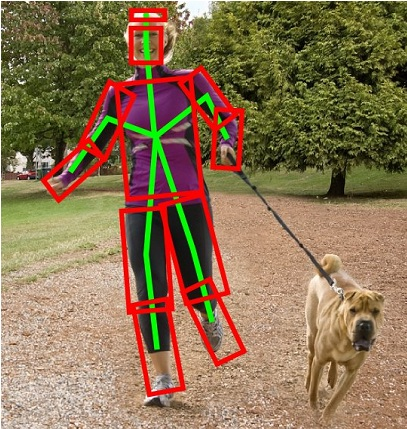
\includegraphics[width=.45\textwidth]{img/graph1.jpg}
    }
    \subfigure[概率图模型表示的图画式结构]{
        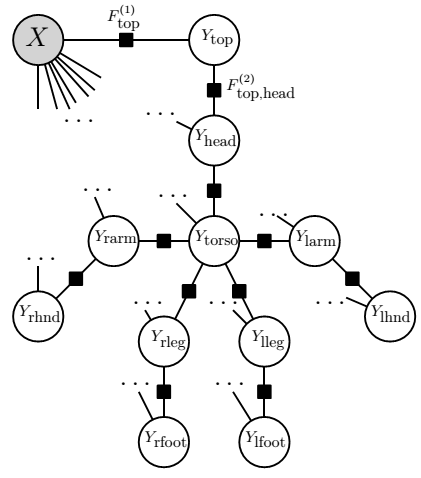
\includegraphics[width=.45\textwidth]{img/graph2.jpg}
    }
    \bicaption{概率图模型}{概率图模型}{Fig}{Graphic Model}
    \label{fig:graphmodel}
\end{figure}


\section{图画式结构}
基于对象的图画式结构模型是由部位的集合构成的,并且包含了部位之间的联系,像一个弹簧结构一样,有些部位之间有关联。
图画式结构模型采用形状特性来描述每个部位,用形变信息来描述相关联的两个部位。
本质上来说,它是一个很通用的模型,因为这个模型和具体描述每个部位的形状特征是无关的,研究者可以使用任意一种形状特征,比如方向梯度直方图(HOG)等,
而且这个模型和描述相关联部位的形变特征也是无关的,研究者也可以使用任意一种形变特征。
一般来讲,表示图画式结构模型的最自然的方式是无向图$G=(V, E)$,其中顶点集合为$V = \left\{v_1, v_2, \cdots, v_n \right\}$,对应了n个部位,
任意一条边$(v_i, v_j) \in E$ 代表了两个相关联顶点$v_i$和$v_j$之间的关系。
对于物体的信息,我们用配置信息$L = (l_1, l_2, \cdots, l_n)$ 来描述,其中$l_i$代表部位$v_i$的位置。
一般情况下,我们的$L$只代表物体的位置,但是配置信息其实还可以代表更多的信息,它代表了每个部位的表示方式。
每个部位的位置信息可以简单的描述它在图像中的像素位置,但是更复杂的、更多的参数也是可能的。
举例来说,对于我们文章中提出的隐式衣服属性模型,每个部位的配置信息包括位置、大小、方向等信息。

\begin{figure}
\centering
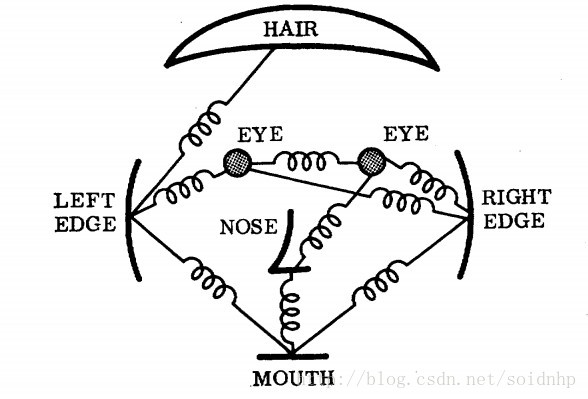
\includegraphics[width=0.9\textwidth]{img/ps.jpg}
\bicaption{人脸部弹簧模型}{人脸部弹簧模型}{Fig}{Pictorial Structure for Face Detection}
\label{fig:ps}
\end{figure}

在图画式结构模型的经典论文\cite{ps1}中,我们用能量函数来描述一个图画式结构模型和测试图片之间的不匹配程度,
而问题就是要最小化这个能量函数。
对于每一种所有部位的配置形式的损失或者能量,它与下面两方面内容有关系:
一是每个部位跟测试图片中这个位置的不匹配程度,而是两个部位的位置关系和形变模型的不匹配程度。
给定一张图片,用函数$m_i(l_i)$来测量部位$v_i$和测试图片中位置$l_i$的不匹配程度。
对于两个相关联的部位,我们用函数$d_{ij}(l_i, l_j)$来测量$(v_i, v_j)$和测试图片中位置$(l_i, l_j)$的不匹配程度。
因此,对于测试图片来说,和模型最匹配的配置信息形式应该是:

\begin{equation}
    \label{eq:pseq}
    L^{\*} = arg \min {\left( \sum_{i=1}^{n} m_i(l_i) + \sum_{ (v_i, v_j) \in E } d_{ij}(l_i, l_j) \right)}
\end{equation}

公式表示了一种最优的配置信息,它最小化了每个部位的不匹配程度$m_i$与每两个关联部位不匹配程度$d_{ij}$的和。
一般地,描述形变特征不匹配程度的函数往往只跟两个部位的相对位置有关系,这样使得模型可以很好的使用全局变换。
需要注意的是,一个图画式结构模型和测试图片的能量函数不只是跟每个单独部位的位置有关系,
而是依赖于所有的部位形状特征匹配度和所有相关联部位的形变特征匹配度的。

\begin{figure}[tbp]
    \centering
    \subfigure[]{
        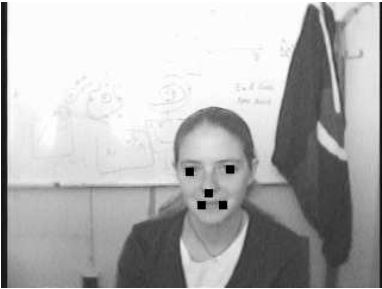
\includegraphics[width=.45\textwidth]{img/ps1.JPG}
    }
    \subfigure[]{
        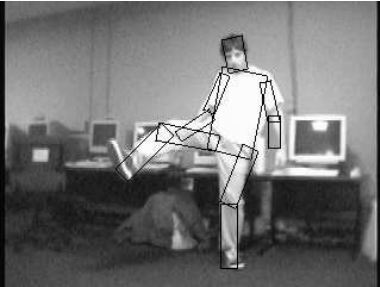
\includegraphics[width=.45\textwidth]{img/ps2.JPG}
    }
    \bicaption{用图画式结构检测出的一个简单的例子,人脸(a)和一个人体(b)。每张图片展示了需要检测的物体的全局最优解,
        这是算法检测出的结果。这个物体模型是从训练数据学习出来的。}{用图画式结构检测出的一个简单的例子,人脸(a)和一个人体(b)。每张图片展示了需要检测的物体的全局最优解,
        这是算法检测出的结果。这个物体模型是从训练数据学习出来的。}{Fig}{Sample results for detection of a face (a); and a human body (b). Each
image shows the globally best location for the corresponding object, as computed by
our algorithms. The object models were learned from training examples.}
    \label{fig:ps2}
\end{figure}


可以看出这个能量函数\ref{eq:pseq}是简单并且直观的。
然而前人的很多工作都是采用启发式的或者局部搜索技术,他们很难找出一个最优解,因为最优解的获得严重依赖于初始化的方式,初始化参数设置的好,那么就有可能获得最优解,否则会很被动。
而图画式结构模型提供了一种高效并且简单的方式,可以找到一个全局的最优解,并且不需要任何初始化步骤。

图画式结构模型不仅可以表示计算机视觉中图片中的人物躯干、脸部器官等,还可以表示更一般的物体。
例如,对于每个部位的外观模型,可以是颜色或者方向特征,或者是局部方向过滤器的响应等,
两个部位之间的关联也可以用更一般的形式来建模,比如“接近”,“在左边”,“在上方”,或者更精确的几何上的约束(比如联合角度)。
因为每个部位的外观模型和任意两个相连部位之间的形变模型都可以一般化,所以图画式结构模型提供了一个强大的框架。
假设我们想对人体躯干的外观特征进行建模,很自然地我们要将人体躯干建模为一系列有关节的部位,并且连接了不同的人体部位。
通过图画式结构模型,我们可以采用一个粗粒度的模型,用数目比较少的部位表示。
简单的部位外观模型和相连部位的形变模型的结合提供了足够的上下文信息来找到人体躯干,但是对于找出更一般的人体部位还是很困难的,还是一个很大的挑战,
比如“小腿”或“上臂”等。

\section{结构式学习}
在计算机视觉领域,从大数据中学习出来的强大的统计模型正在不断的改进。
这些模型都包含了一个丰富的内部结构,来反映真实问题中任务相关的变量之间的关系和约束。
本节主要介绍下一些在计算机视觉领域非常流行的结构化模型,更为精确的是基于离散变量的无向图模型,它可以表示一大类算法描述,
比如概率预测和最大化后验概率。
下面我们主要来看一下结构式学习在计算机视觉领域的应用。


一般来讲,计算机视觉的目的就是让计算机能够从图片数据中理解出更高层的语义信息。
这些图片数据可能来自于各种种类的格式或者形式,它可以是一张自然图片,也可以是多张卫星图片序列,沿着时间序列拍摄的。
同样地,我们所讲的高层次信息也是多种多样的,从像素级别的图片表面信息,到图片中一般的物体(比如车、动物等)级别的信息。

\begin{figure}
\centering
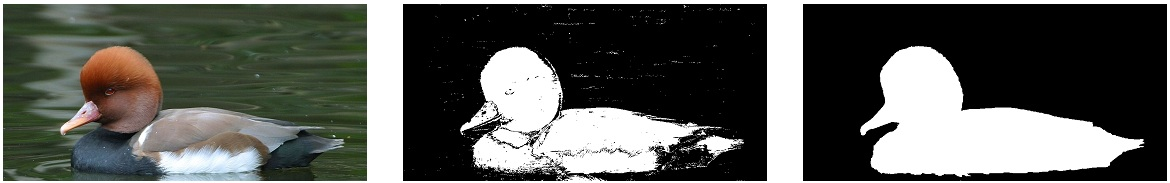
\includegraphics[width=0.9\textwidth]{img/struct.jpg}
\bicaption{首先第二幅图是利用简单的前背景和后背景分类器就可以输出,
而第三幅图必须使用像素之间的关联才可以做到图像分割。}{首先第二幅图是利用简单的前背景和后背景分类器就可以输出,
而第三幅图必须使用像素之间的关联才可以做到图像分割。}{Fig}{Pixel-wise separate classification by pixel only: 
noisy, locally inconsistent decisions. Joint optimum result with spatially consistent decisions.}
\label{fig:struct}
\end{figure}

上述所讲的任务一般会构建一个模型,这个模型是跟图像数据和高层次信息都有关的一个模型。
这个模型中包含了一组变量的集合,其中包括可观测的用来描述图片数据的变量,描述高层次信息的输出变量,
还有一类辅助变量,用来描述输入输出之间的关系等。
在这些变量之外,模型还定义了变量之间是怎么互相关联的,如何互相依赖的等。
这些变量和变量之间的关系构成了这个模型的结构。
结构化模型允许我们构建任意多的变量和变量之间的关联信息,从而可见结构化模型的表征能力是极其强大的,它可以表达出非常复杂的关系,
图像数据和任意感兴趣的高层次信息之间的关系,都可以用结构化模型来表征。

不止于构建一个单一的固定模型,我们还可以增加参数来描述变量之间的关系。
给定标记好的数据和已知的输出变量类型,我们可以调整模型的参数,从而学出一组使得观测变量和输出变量最匹配的参数。这即就是参数学习或模型训练。

\begin{figure}
\centering
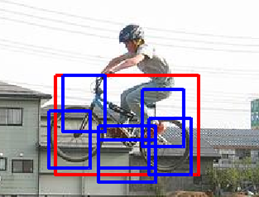
\includegraphics[width=0.7\textwidth]{img/dpm1.png}
\bicaption{自行车的检测案例}{自行车的检测案例}{Fig}{Example for bicycle detection.}
\label{fig:dpm1}
\end{figure}

\section{形变部位模型}
形变部位模型\cite{llsvm}DPM(Deformable Part Model)是一个非常成功的目标检测算法,
连续获得VOC(Visual Object Class)07,08,09年的检测冠军。
目前已成为众多分类器、分割、人体姿态和行为分类的重要部分。
2010年Pedro Felzenszwalb被VOC授予“终身成就奖”。
DPM可以看作是HOG(Histograms of Oriented Gradients)的扩展,大体思路与HOG一致。
先计算梯度方向直方图,然后用SVM(Support Vector Machine)训练得到物体的梯度模型(Model)。
有了这样的模板就可以直接用来分类了,简单理解就是模型和目标匹配。DPM只是在模型上做了很多改进工作。

\begin{figure}
\centering
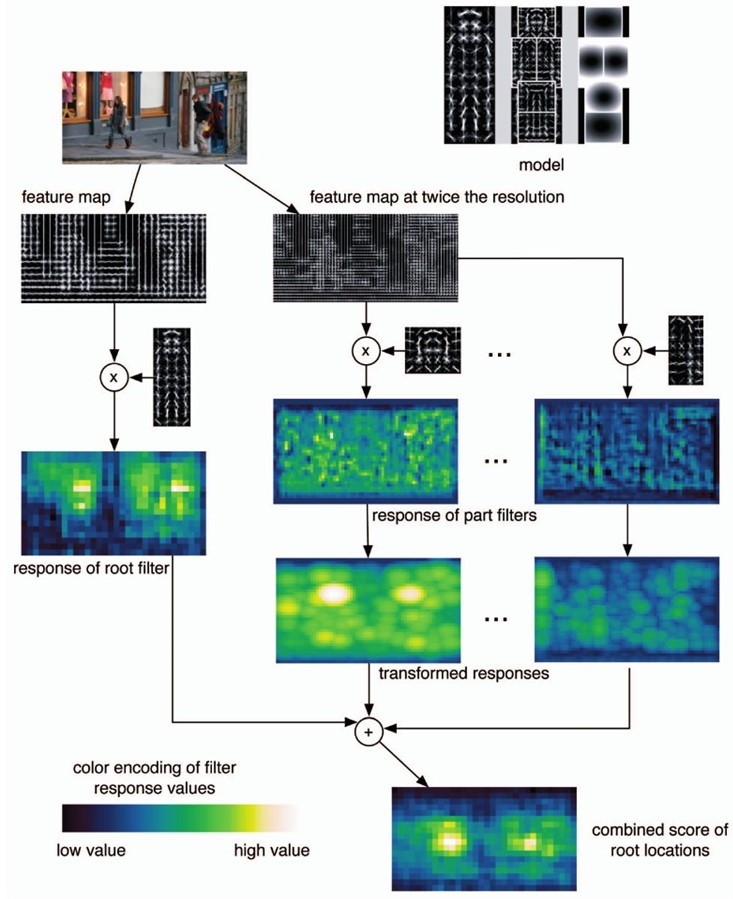
\includegraphics[width=0.9\textwidth]{img/dpm.jpg}
\bicaption{DPM模型的框架流程图}{DPM模型的框架流程图}{Fig}{The framework for DPM model}
\label{fig:dpm}
\end{figure}

上图是HOG论文中训练出来的人体模型。它是但模型,对直立的正面和背面人检测效果很好,较以前取得了重大的突破。
也是目前为止最好的特征(最近被CVPR2013年的一篇论文\cite{hsc}超过了)。
但是,如果是侧面呢,所以自然我们会想到利用更多的模型去构建。
DPM就使用了2个模型,主页上最新版本的程序使用了12个模型。
有了多模型,就可以解决视角的问题了,还有一个严重的问题,动物是动的,就算是没有生命的车也有很多款式,
单单有一个模型,如果动物动一下,人物运动一下,那模型就跟这个人的匹配程度就低了很多。
也就是说,我们的模型适应能力太差了,不能适应物体的运动,特别是非刚性物体的运动,自然我们又能想到添加子模型,比如给手一个子模型,
当手移动时,子模型能够检测到手的位置。把子模型和主模型的匹配程度综合起来,最简单的就是相加,那模型匹配程度就会提高。
还有我们要加入子模型和主模型中位置的偏移程度的损失,也就是综合得分要减去偏移的损失。
本质上就是要使用子模型和主模型的空间先验知识。



\section{本章小结}
本章介绍了与我们工作相关的一些背景知识,包括图模型、图画式结构模型、结构式学习、形变部位模型等。
图模型是我们算法的基础,它定义了一个非常强大的语言,将我们实际问题中变量的关系表示的非常清楚,
它表征了变量之间的概率关系,特别适合复杂问题的变量关系表示。
图画式结构模型提供了一个弹簧结构问题的优化算法,基于图模型将变量之间的关系通过一种特殊的结构构建起来,
特别适用于人体结构预测、人脸特征部位预测等实际问题。
结构式学习是很多机器学习问题的基础,它可以解决很多复杂问题,
包括自然语言处理中的问题,计算机视觉中的问题,语音识别中的问题等。
形变部位模型是近年来物体识别领域最火的一个模型,它为本文的工作提供了一个基础的想法框架。
通过对这些模型的介绍,使得对我们工作的背景和动机有一个清晰明确的认识,并且有助于对人体姿势预测整个领域有一个深入的了解,
并且有助于理解我们在本文中提出的模型算法。


% our model
% !Mode:: "TeX:UTF-8"
%%==========================
%% chapter01.tex for SJTU Master Thesis
%% based on CASthesis
%% modified by wei.jianwen@gmail.com
%% version: 0.3a
%% Encoding: UTF-8
%% last update: Dec 5th, 2010
%%==================================================

%\bibliographystyle{sjtu2} %[此处用于每章都生产参考文献]
\chapter{基于隐式衣服属性变量的姿势预测}
\label{chap:model}

\begin{figure}[tbp]
\centering
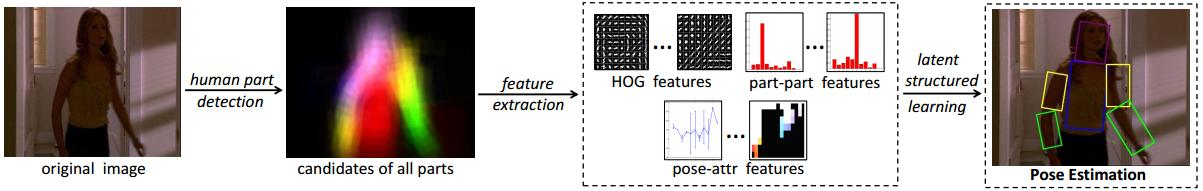
\includegraphics[width=\textwidth]{img/frame.pdf}
\caption{ \textbf{我们算法的框架} }
\label{fig:frame}
\end{figure}

在图\ref{fig:frame}中,我们描述了我们提出的方法。
首先,我们进行一步预处理,检测出图片中可能的人体姿势,构成一个人体姿势解的候选集。
这使得我们可以对搜索空间进行管理,从而降低我们的搜索空间,加速我们的求解过程。
其次,我们设计并抽取了人体部位和衣服属性相关的特征。
接着,我们采用隐变量结构式支持向量机框架进行模型参数的学习,
最后,我们设计了一个高效的预测算法来求得人体部位和衣服属性的近似最优解。
需要注意的是,我们的方法最后也给出了一个精确的衣服属性类别,这样可以将具有相似衣服属性的图片聚集在一起。
这也是我们有贡献的一步。


\begin{table}
\label{tb:attr}
\centering
\caption{人体躯干和衣服属性的关系}
\begin{tabular}{|c|c|c|c|} \hline
衣服属性& 人体部位& 底层特征& 类别数目\\ \hline
Sleeve &  All arms & Color Histogram & 3 \\ \hline
Neckline & Torso + Head & HOG & 4\\ \hline
 Pattern & Torso & LBP~\cite{lbp} & 5\\ \hline
\end{tabular}
\end{table}

在介绍我们的模型细节之前,我们介绍一些本文中需要用到的符号表示。
我们用$I$来表示一副图片,用一个矩形框$(x, y, s, \theta)$ 来表示一个人体部位,
$(x, y)$是人体部位的坐标,$s$是大小,$\theta$是人体部位的倾斜度。
假设我们一副图片中有$m$个人体部位(在本文中,$m = 6$)。
为了使模型输入的搜索空间在一个可控的范围内,我们采用目前结果最好的方法为每个人体部位产生40个候选解。因此我们问题的输入空间可以表示为:
\begin{equation}
    \mathcal{X} = \left\{ \mathbf{x}|\mathbf{x} = ( \mathbf{b}_1, \mathbf{b}_2, \cdots, \mathbf{b}_m ) \right\},
\end{equation}

对于一个图片$\mathbf{x}$,$\mathbf{b}_i$表示第i个人体部位的候选解集(包含40个候选解)。
而我们人体姿势的输出空间为:
\begin{equation}
    \mathcal{P} = \{\mathbf{p}| \mathbf{p}=(p_1,p_2,\cdots,p_m), \forall i, 1\leq p_i \leq 40\},
\end{equation}
$p_i$ 是一个下标,它表示候选解集$\mathbf{b}_i$中第i个元素的下标。

我们的目的是将衣服属性加入到人体姿势预测问题中,
通过捕捉到人体部位与衣服属性之间的关系。
在本文中,我们考虑了三种衣服属性,包括Neckline(衣领样式)、Pattern(衣服纹理)和Sleeve(袖子)。
对于每一个衣服属性来说,它会有多个样式,比如袖子属性有长袖、短袖和无袖等。
在表\ref{tb:attr}中,我们对于每一个衣服属性,根据经验定义了它的类别数。
因此我们问题中衣服属性的输出空间为:
\begin{equation}
    \mathcal{A} = \left\{ \mathbf{a}|\mathbf{a} = (a_1, a_2, \cdots, a_n), \forall r, 1 \leq a_r \leq T_r \right\}.
\end{equation}

$n$ 是衣服属性的个数(本文中,$n = 3$),$a_r$ 是第$r$个属性的类别标签。
需要注意的是,我们并不知道这些属性的类别标签的具体含义,比如$a_1 = 1$可能代表短袖,也可能代表长袖。
因为在本文中,识别衣服属性是一个聚类问题,我们只把具有相似衣服属性类别的图片样本聚集到一起。

因此我们的问题(基于隐变量衣服属性的人体姿势预测)可以形式化为一下式子:
\begin{equation}
    f: \mathcal{X} \rightarrow \mathcal{Y},
    \label{eq:task_func}
\end{equation}
其中 $\mathcal{Y}$ 是我们问题的输出空间,它被定义如下:
\begin{equation}
    \mathcal{Y} = \left\{ \mathbf{y}|\mathbf{y} = (\mathbf{p},\mathbf{a}), \mathbf{p} \in \mathcal{P}, \mathbf{a} \in \mathcal{A} \right\},
\end{equation}

考虑预测函数 $f$,我们假定有一个分数函数 $S$ 定义了输入-输出对 $(\mathbf{x}, \mathbf{y})$ 的匹配程度:
\begin{equation}
\label{eq:map}
    S(\mathbf{x}, \mathbf{y};\beta) = \langle \beta, J(\mathbf{x}, \mathbf{y}) \rangle
\end{equation}

其中 $\langle \cdot \rangle$ 表示两个向量的内积,
$J(\cdot, \cdot)$ 是我们问题的联合特征表示,
$\beta$ 是需要去学习的模型参数。

因此,我们的匹配函数 $f$ 可以写为如下表示:
\begin{equation}
    f(\mathbf{x}; \mathbf{\beta}) = arg \max_{ \mathbf{y} \in \mathcal{Y} } S(\mathbf{x}, \mathbf{y}; \mathbf{\beta})
    %f(\mathbf{x}; \mathbf{\beta}) = \argmax { \mathbf{y} \in \mathcal{Y} } S(\mathbf{x}, \mathbf{y}; \mathbf{\beta})
    \label{eq:score}
\end{equation}
这是一个包含隐变量的结构式学习问题,其中衣服属性是隐变量。
我们模型的学习过程是来自于\cite{dpm}这篇文章的启发,是一个不断调整的策略,来提升隐变量的预测精度。


在本章中,我们将描述我们提出的模型,这是一个典型的结构式学习(structure learning)问题。
我们将分为三部分来描述我们的模型。
第一部分是联合特征的分析与设计,这是所有结构式学习问题中很关键的一步,因为设计好了特征,才有可能使得我们的模型达到一个比较好的结果。
我们设计的特征既包含了人体部位的特征,也包含了人体部位与衣服属性的联合特征,这样我们将衣服属性的特征很好的结合到传统的人体姿势预测问题中。
第二部分是基于隐变量的结构式学习,这是我们模型的参数学习过程。
其中包含了多个问题的解决方案,包括隐变量的初始化,负样本空间的管理,以及模型训练的策略问题。
模型参数的学习也要用到第三部分的预测算法,因为模型训练过程中,需要调用预测算法来估计局部最优解,进而得到正样本。
第三部分是基于模型的有环图预测算法,这部分的输入是训练好的模型和一张新的测试图片,输出是人体姿势和衣服属性的最优解。
下面我们详细介绍每一部分。

\section{联合特征分析与设计}
联合特征的设计是所有结构式学习中比较关键的一步\cite{svm-struct},特征设计的好坏关系到模型预测能力的好坏,并决定了模型预测能力的上限。
我们设计了两类特征来构成我们问题的联合特征$J(\mathbf{x}, \mathbf{y})$,包括人体姿势相关的特征$j_p(\mathbf{x}, \mathbf{p})$,以及人体姿势和衣服属性相关的特征$j_{pa}(\mathbf{x}, \mathbf{y});$。

总体来看,我们问题的联合特征表示如下:
\begin{equation}
    \label{eq:feature}
    \langle \mathbf{\beta}, J(\mathbf{x},\mathbf{y}) \rangle = \langle \mathbf{\beta}_p, j_p(\mathbf{x}, \mathbf{p}) \rangle + \langle \mathbf{\beta}_{pa}, j_{pa}(\mathbf{x},\mathbf{y}) \rangle
\end{equation}
下面,我们详细介绍我们是如何设计每一类特征的。




\begin{algorithm}
\caption{包含隐变量的结构式支持向量机学习}
\begin{algorithmic}[1]
    \REQUIRE 正例样本集合, 负例样本集合, 初始模型参数 $\beta$, 重调整策略的次数 $t_1$, 困难负例挖掘的迭代次数 $t_2$.
    \ENSURE 最终模型 ${\beta}^*$.
    \STATE 初始化最终模型: ${\beta}^* = \beta$.
    \STATE 标记负例集为 $F_n = \emptyset$.
    \FOR{ relabel = 1 to $t_1$ }
        \STATE 标记正例集为 $F_p = \emptyset$.
        \STATE 将正例逐个加入 $F_p$.
        \FOR{ iter = 1 to $t_2$ }
            \STATE 将负例逐个加入 $F_n$.
            \STATE ${\beta}^* := \mathrm{Pegasos}({\beta}^*, F_p \bigcup F_n)$.\\
            \STATE 将容易的负例去除掉: \\
             删除掉那些负例特征 $v$ 满足 $\langle{\beta}^*, v \rangle < -1$ from $F_n$.
        \ENDFOR
    \ENDFOR
\end{algorithmic}
\label{alg:train}
\end{algorithm}


\subsection{人体躯干相关特征}
对于一个输入样本$\mathbf{x}$,我们用方向梯度直图(HOG)\cite{hog} 来描述一个候选解的形状,
而且我们考虑了两个相连的人体躯干之间的形变约束关系:
\begin{equation}
    j_p(\mathbf{x}, \mathbf{p}) = \sum_{i=1}^m hog(\mathbf{x}, p_i) + \sum_{(i, j) \in E_p} d(\mathbf{x}, p_i, p_j),
\end{equation}
其中$E_p$ 是相连人体躯干的集合。

形变特征的设计主要考虑相连人体躯干之间的几何约束,包括相对位置、相对角度和两者的距离,计算公式为:
$[x_j - x_i, y_j - y_i, (x_j - x_i)^2, (y_j - y_i)^2]$~\cite{deva11}.

\subsection{衣服属性相关特征}
通过衣服属性特征,我们将衣服属性结合到我们模型当中。
需要注意的是,一个衣服属性可能会关联多个人体躯干,比如袖子会关联到所有的手臂躯干。
对于一个给定的属性 $r$,我们用 $r_p$ 来表示跟属性 $r$ 相关的人体躯干,用 $P_r$ 来表示这种对应关系的配置信息。
在表 \ref{tb:attr} 的第二栏中,我们给出了衣服属性和人体躯干之间的对应关系。
显而易见,对于不同的衣服属性,应该使用不同的底层特征来描述,这样才能达到很好的特性 \cite{clothliu}。
我们在表 \ref{tb:attr} 的第三栏给出了这种对应关系,每种衣服属性对应的底层特征。

因此衣服属性特征可以形式化为:
\begin{equation}
    \label{eq:j_pa}
    j_{pa}(\mathbf{x}, \mathbf{y}) = \sum_{r=1}^n \Psi(\mathbf{x}, P_r, a_r)
\end{equation}
其中 $\Psi(\mathbf{x}, P_r, a_r)$ 表示从样本 $x$ 中抽取出来的关于 人体躯干的对应配置 $P_r$ 和衣服属性类别 $a_r$ 的衣服属性特征。


跟之前的工作\cite{shen2014unified}类似,我们将衣服属性特征设计为底层特征和属性类别向量的外积,这样可以采用一种简单有效的方式将人体躯干和衣服属性联合起来。
首先,我们将衣服属性的类别标签 $a_r$ 转化为一个维度是 $T_r$ 的向量 $L(a_r)$,
在这个向量里,只有一维数据是1,其余都是0。
根据表 \ref{tb:attr},第$r$个衣服属性的底层特征依赖于下述两方面:
衣服属性对应的人体躯干和衣服属性标签。
我们用$F_r(P_r)$来表示第$r$个衣服属性对应的特征,并且跟衣服属性对应的人体躯干配置 $P_r$ 有关。

因此,我们的衣服属性特征 $\Psi(\mathbf{x}, P_r, a_r)$ 可以表示为以下式子:
\begin{equation}
    \Psi_{pa}(\mathbf{x}, P_r, a_r) = F_r(P_r) \otimes L(a_r)
\end{equation}
其中的符号操作 ``$\otimes$'' 表示将两个向量的外积之后的矩阵向量化。

\section{基于隐变量的结构式学习}
在上节中,我们设计了问题的联合特征,现在我们来考虑模型的训练问题。
我们的训练数据集有人体姿势的标签信息,这是人体姿势预测问题的所有标准数据集都拥有的数据信息。
但是数据集中没有衣服属性的标签信息,我们通过把衣服属性作为隐变量的方法去训练模型。

在本节中,我们提出了一个框架用来初始化这个结构式问题和学习所有的参数。
我们将问题的参数学习部分转化为一个LSSVM(Latent Structure Support Vector Machine,隐变量结构式支持向量机)训练问题来进行求解。
对于一个LSSVM问题,我们设计了一种重标记的方式来求解,并且结合数据挖掘(困难数据挖掘)技术来控制负样本空间的大小,
并且我们采用Pegasos\cite{pegasos}算法来进行在线学习,这样就可以解决因为负例空间巨大而造成的训练时间复杂度很大。

\begin{algorithm}
\caption{衣服属性预测算法}
\begin{algorithmic}[1]
    \REQUIRE 测试图片样本 $\mathbf{x}$, 模型参数 $\beta$ , 人体姿势的局部最优解 $\mathbf{p}$
    \ENSURE 衣服属性的最优解 $\mathbf{a^*}$
    \STATE 用 $T_r$ 来标记第 $r$-th 个衣服属性的种类数量
    \FOR {r:= 1 \textbf{to} 3}
        \STATE 选择使得下列分值函数值最高的衣服属性类型:\\
            %$\mathbf{a}_r = \argmax_{1 \leq r \leq T_r} \langle \beta_{pa}^r, j_{pa}(\mathbf{x}, P_r, a_r) \rangle $
            $\mathbf{a}_r = arg \max_{1 \leq r \leq T_r} \langle \beta_{pa}^r, j_{pa}(\mathbf{x}, P_r, a_r) \rangle $
    \ENDFOR
\end{algorithmic}
\label{alg:attr}
\end{algorithm}


\subsection{目标函数}
在这一小节中,我们需要定义问题的目标函数,即就是问题的优化函数,通过对优化函数的训练而求得我们最终的解。
而我们的优化函数目标是学习我们在式\ref{eq:map}中定义的匹配函数 $S(\mathbf{x}, \mathbf{y}; \beta)$,它将在后面联合估计预测中用到。
给定一个正例训样样本 $(\mathbf{x}, \mathbf{y})$,我们期望匹配函数 $S(\mathbf{x}, \mathbf{y}; \beta) \geq 1$。
另一方面,如果一个训练样本是负例,那么匹配函数的输出应该是小于$-1$的。
因此,给定一个训练集 $D = \{ (\mathbf{x}_1, \mathbf{y}_1, z_1), \cdots, (\mathbf{x}_q, \mathbf{y}_q, z_q) \}$, 其中 $z_k \in \{1, -1\}$ 表示第 $k$ 个样本是正例还是负例,我们可以通过优化以下函数来求解模型的参数 $\beta$:
\begin{equation}
\begin{split}
\min_{\beta}  \frac{1}{2} \|\beta\|^2 + C \sum_{k=1}^{q}\max(0, 1 - z_k S(\mathbf{x}_k, \mathbf{y}_k; \beta)).
    \label{eq:latent}
\end{split}
\end{equation}

\subsection{隐变量初始化}
对于一个包含隐变量的结构式学习问题,隐变量的初始化是关键的一个步骤。
在本问题中,衣服属性是作为隐变量的,而人体躯干对于我们来说是观察量,是有标签信息的。
为了模型的初始化,我们采用一种重标记的策略来更新正例中衣服属性的标签信息和模型参数$\beta$。

有很多种方式可以进行模型中隐变量的初始化,我们可以随机的为隐变量设定标签信息,但是很有可能造成模型的不稳定性。
在本文中,我们首先根据人体躯干的标签信息抽取每个衣服属性对应的底层特征,
然后采用$k$-Means聚类算法来获得每个衣服属性的类中心,
其中 $K$ 是我们在表\ref{tb:attr}中定义的衣服属性的类别数目。
因此,隐变量衣服属性的初始标签可以通过其最近的类中心来决定。
通过这种初始化的方式,我们得到了所有衣服属性的初始标签信息,所以我们可以求解问题 \eqref{eq:latent} 来得到初始的模型参数 $\beta$。

\subsection{模型训练策略}
由于初始化的衣服属性类别信息不够精确,我们采用一种重标记的策略来不断更新衣服属性值。
即就是,当给定了模型的参数 $\beta$ 和人体躯干的标签信息后,我们通过最大化匹配函数 $S(\mathbf{x}, \mathbf{y}; \beta)$ 来预测衣服属性的标签信息,计算细节在算法 \ref{alg:attr} 中。
需要注意的是,根据我们联合特征的设计规则来看,衣服属性的预测与人体躯干的特征无关的,它只与衣服属性特征有关。

根据公式\eqref{eq:j_pa},我们可以看出不同衣服属性之前是没有交集的,因为 $j_{pa}$ 是 $n$ 个独立衣服属性关联的特征的连接。
因此,我们可以通过一个高效的贪心搜索算法来求得每一个衣服属性的局部最优解(算法\ref{alg:attr}第2到4行)。


\subsection{负样本空间管理}
对于一个识别或者检测的任务,我们可以获得一个大小可控的正例样本集。
然后,对于负例集来说,样本空间会非常大,因为任意给正例样本加一些误差就可以得到一个负例。
实际上,我们是不可能枚举所有的负例样本。
因此,我们很有必要设计一个算法来控制负例样本集合的大小,这样才能使得模型高效并且节省内存消耗。
在算法\ref{alg:train}的第6--10行,我们采用困难负例挖掘\cite{dpm}的技术来获得有效的负例样本。
这一步将会调用预测算法\ref{alg:inference} (见章节\ref{subsec:inference})。
更加详细的说,给定一个输入样本$\mathbf{x}$和模型参数$\beta$,我们采用预测算法\ref{alg:inference}来找到局部最优解$\mathbf{y}^*$。
如果 $z \cdot S^*$ 小于 $-1$ (我们设定的一个阈值),那么我们认为样本$\mathbf{x}$是困难负例。
我们的算法将会停止对样本$\mathbf{x}$的最优解搜索,只有到$S^*$ 大于 $-1$ 时才会继续加入搜索集合(前一步得到解$\mathbf{y}^*$将会从搜索空间中删除)。

在收集了所有的困难负例样本以后,我们会用Pegasos算法\cite{pegasos}来更新模型的参数(见算法\ref{alg:train}第8行)。
然后我们采用更新后的模型参数去从负例样本集合中删除那些困难样本。


\begin{algorithm}
\caption{包含隐变量衣服属性的HPE近似预测算法}
\begin{algorithmic}[1]
    \REQUIRE 测试图片样本 $\mathbf{x}$, 模型参数 $\beta$.
    \ENSURE 人体姿势的最优解 $\mathbf{y}^*$ 和最优分值 $S*$.
    \STATE Set $\mathbf{y}^* = \emptyset$.
    \STATE 记最优的分值为 $S^* = -\infty$.
    \STATE 初始化人体部位最优解 $\mathbf{p}_0$.
    \REPEAT
        \STATE 计算局部衣服属性最优解 $\mathbf{a}_t$.
        \STATE 计算局部人体姿势最优解 $\mathbf{p}_t$.

        \STATE 计算局部最优分值: $S = S(\mathbf{x}, \mathbf{y}_t; \beta)$.

        \IF{$S > S^*$}
            \STATE $S^* = S$, $\mathbf{y}^* = \mathbf{y}_t $
        \ENDIF
    \UNTIL{$S^*$ 不再变化}
\end{algorithmic}
\label{alg:inference}
\end{algorithm}


\begin{figure}[tbp]
\centering
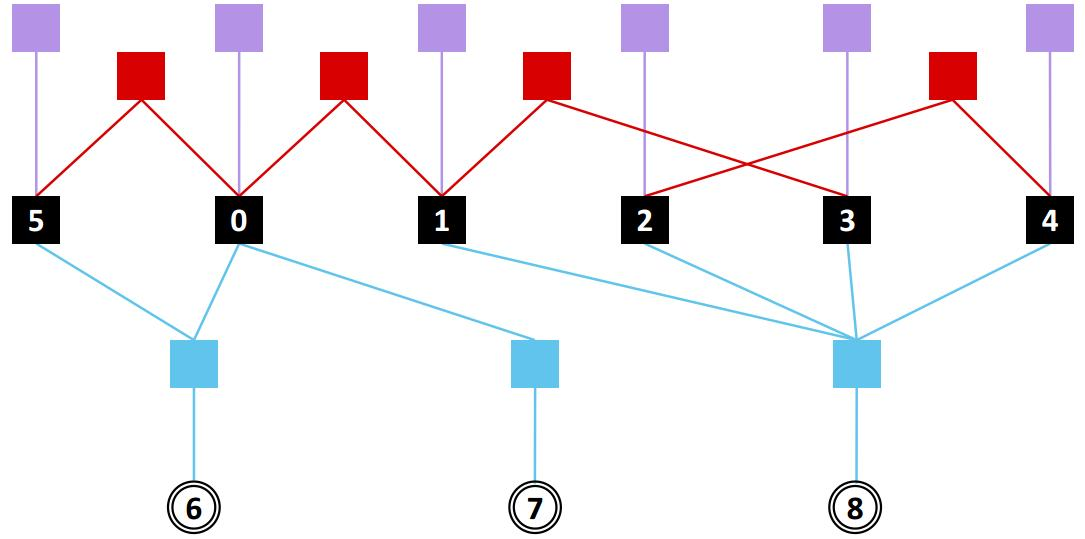
\includegraphics[width=0.9\textwidth]{img/whole-model.pdf}
\caption{ \textbf{我们问题的因子图表示} }
\label{fig:graph}
\end{figure}

\section{有环图的预测}
\label{subsec:inference}

\subsection{因子图表示}
在图\ref{fig:graph}中,我们将问题用因子图去描述。
因为实际上我们的问题是一个图模型问题,变量之间有依赖关系,而因子图就是图模型问题中描述变量之间关系的最好方式。
其中,黑色矩形节点表示人体躯干变量,双环圆形节点表示衣服属性变量,其它颜色的方块表示变量之间的依赖关系。
从因子图\ref{fig:graph}可以看出,我们问题的结构是一个有环图,这样就不能用传统的图画式框架算法进行精确高效的优化预测。
因此在算法\ref{alg:inference},我们提出了一个高效的预测算法,来通过坐标下降的方式来求得近似最优解。
算法\ref{alg:inference}的输入是一个测试样本 $\mathbf{x}$ 和模型参数 $\beta$,输出为人体躯干和衣服属性的局部最优解。
具体来说,在每一步迭代中,当衣服属性变量固定时,问题的结构可以变为一个树结构(无环图),这可以通过动态规划算法\cite{ps2}进行优化。
当人体躯干变量固定时,我们可以通过一个高效的贪心算法来求得局部最优解(详见算法\ref{alg:attr})。

\subsection{最优解估计}
%\subsection{人体躯干的预测}
这一小节,我们来介绍一下人体躯干的预测算法。
之前我们提到过,我们的问题结构是一个有环图,但是当衣服属性变量固定时,我们可以进行一个拆换操作。
具体来说,就是将衣服属性节点作为其相关人体躯干变量节点的子节点,这样就构成一个无环树状图。
因此,我们在传统的图画式结构算法框架上进行了扩展改进,提出一个新的扩展版图画式算法来解决这个有环图问题。
在图\ref{fig:graph}中,我们用不同颜色的节点来表示变量之间的依赖关系分值,
紫色节点代表关于形状的分值,红色节点代表关于形变的分值。
淡绿色的节点代表了我们扩展版图画式算法的主要核心部分,它表示了每个衣服属性变量和其对应的人体躯干之间的依赖关系分值。
因此,我们在算法\ref{alg:ps}中描述了我们的人体躯干预测算法。
我们用符号 $C_i$ 来表示节点 $i$ 的子节点。
在算法\ref{alg:ps}的第3--5行,我们计算了关于形状的分值和衣服属性特征的分值。
在第7行,我们计算出了父子节点之间对应的依赖关系分值。
在第8--12行中,我们采用动态规划计算了节点之间的分值传递过程,每步中父亲节点的分值依赖于所有子节点的分值。
接着在第14--17行中,我们采用了一个自顶向下的方法来找到每一个人体躯干的最优候选解。
通过以上步骤,我们就求得了人体躯干的最优解。

\begin{algorithm}
\caption{人体姿势的预测算法}
\begin{algorithmic}[1]
    \REQUIRE 测试图片样本 $\mathbf{x}$, 模型参数 $\beta$ ,  衣服属性的类别标签值 $\mathbf{a}$
    \ENSURE 人体姿势的最优解 $\mathbf{p^*}$
    \STATE 记人体姿势的最优解集为 $\mathbf{p^*} = \emptyset$
    \STATE 记节点0为根节点
    %\STATE Perform the bottom-up process to compute the score cost for each candidate
    \FOR{ 对于节点 $i$ 的每个候选解 $\mathbf{p}_i$  }
        \STATE 记 $m(\mathbf{p}_i) = \langle \beta_p^i, \phi_p(\mathbf{x}, p_i) \rangle + \langle \beta_{pa}^r, \Psi_{pa}(\mathbf{x}, P_r, a_r) \rangle$
    \ENDFOR
    \FOR{ 对于父亲节点 $j$ 和 $\mathbf{p}_i$ 的子节点 $i$ 的每个候选解 $\mathbf{p}_j$  }
        \STATE set $l(\mathbf{p}_i, \mathbf{p}_j) = \langle \beta_p^{ij}, \psi_p(\mathbf{x}, p_i, p_j) \rangle$
        \IF{ $i$ 是一个叶子节点 }
            \STATE $B_i(\mathbf{p}_j) = \max_{\mathbf{p}_i} (m(\mathbf{p}_i) + l(\mathbf{p}_i, \mathbf{p}_j) )$
        \ELSE
            \STATE $B_i(\mathbf{p}_j) = \max_{\mathbf{p}_i} (m(\mathbf{p}_i) + l(\mathbf{p}_i, \mathbf{p}_j) + \sum_{v \in C_i} B_v(\mathbf{p}_i) )$
        \ENDIF
    \ENDFOR
    %\STATE perform the top-down process to find the best candidate for each human part
    \STATE 为根节点找出最优的解: \\
        $\mathbf{p}_0^* = \arg \max_{\mathbf{p}_0} ( m(\mathbf{p}_0) + \sum_{v \in C_0} B_v(\mathbf{p}_0) )$
    \FOR{ 对于每个父亲-孩子节点对 ($\mathbf{p}_j^*, \mathbf{p}_i$) }
        \STATE $\mathbf{p}_i^* = \arg \max_{\mathbf{p}_i} B_i(\mathbf{p}_j^*)$
    \ENDFOR
\end{algorithmic}
\label{alg:ps}
\end{algorithm}

\section{本章小结}
本章是我们论文最核心的一章,详细描述了本文中提到的基于隐变量衣服属性的人体姿势预测方法。
主要分为三部分,一是联合特征设计,二是模型参数学习,三是有环图预测方法。
联合特征设计是我们算法框架第一步,也是比较关键的一步。
模型参数学习中,我们采用含有隐变量的结构式学习算法,由于包含了隐变量,优化函数变为了非凸函数,
所以不能直接采用梯度下降方法。我们采用迭代式算法来求得近似解。
在预测算法中,我们问题结构变为了有环图,对于无环图我们可以很高效的采用动态规划算法来求得全局最优解,
但是对于有环图,我们无法直接求得全局最优解,于是我们提出了迭代地固定一类变量,来求解另一类变量的局部最优解,
从而求得整个问题的局部最优解。



% !Mode:: "TeX:UTF-8"
%%==========================
%% chapter01.tex for SJTU Master Thesis
%% based on CASthesis
%% modified by wei.jianwen@gmail.com
%% version: 0.3a
%% Encoding: UTF-8
%% last update: Dec 5th, 2010
%%==================================================

%\bibliographystyle{sjtu2} %[此处用于每章都生产参考文献]
\chapter{人体姿势预测的应用案例}
\label{chap:app}
人体姿势检测是计算机视觉领域非常基础的一项工作,我们可以利用人体姿势预测的结果来解决很多其它实际问题,比如基于图片数据集相关的问题,
特别是那些专注在人物相关的问题。
在本章中,首先我们会介绍一下我之前的一篇事件挖掘的工作,我们的工作是基于图片数据集,从Flickr上抓取的人物日常生活照片。
由于以图片数据集作为背景,而且Flickr上的图片数据大部分是包含人物的,而事件挖掘就是要分析图片要表达的语义信息,
所以自然可以想到,我们可以利用人体姿势预测的结果来分析出图片中人物所表达的语义信息,从而进行事件挖掘。
其次,我们会介绍一下人体姿势预测在电商平台上(淘宝、亚马逊、eBay等)衣服搜索的应用。
服饰类商品在电商平台上占据了大量的份额,因此如何帮助人们尽快的找到自己喜欢的衣服是一个很大的挑战,
衣服搜索这项人物应运而生,它的核心就在于分析出图片中衣服的属性信息,然后通过属性信息去海量的衣服数据库中找出最匹配用户需求的衣服。
显而易见,人体姿势预测的结果很明显可以帮助我们去分析出图片中衣服的属性信息,从而进行衣服属性匹配,得到衣服搜索的结果。
最后,我们会介绍一下基于图片的广告推荐。
广告推荐是互联网界最热门的话题之一,它是很多互联网公司最赚钱的部门,广告推荐质量的好坏直接影响到公司整个财年的好坏。
很多传统的广告是基于文本信息,但是随着图片时代的到来,基于图片的广告推荐成为了我们当下最大的挑战。
特别是对于包含人物的图片,我们可以根据周围的语义信息,来推荐合适的产品,从而提高广告推荐的质量,进而为公司带来可观的收入。
下面我们以此来介绍人体姿势预测在这三个任务中的应用。

\section{基于多媒体数据的事件挖掘}
事件挖掘一直是很热门的一个课题,早在70年代就被提出,用来挖掘预测社会上的突发事件,比如地震、恐怖事件等。
随着互联网时代的到来,信息的产生和传播变得越来越迅速,互联网上发生了很多很多事情,如何快速的去挖掘甚至预测事件,是一个很大的挑战。
我们之前的一份工作就是考虑在社交图片分享网站Flickr上的事件挖掘问题。
Flickr目前是全球最大的图片社交分享网站,每天有大量的用户在上面分享图片,记录自己的个人生活,而这些图片里实际上包含了大量的事件信息。
比如奥运会、比赛、个人旅游等照片,如果我们能挖掘出其中的事件信息,那么对于用户图片的组织,甚至搜索引擎中结果的结构化展示都有极其强大的帮助。

\begin{figure}
\centering
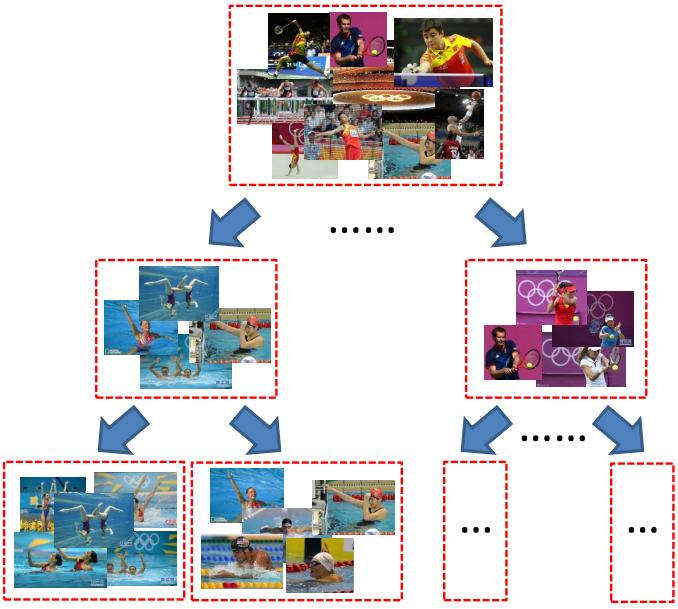
\includegraphics[width=0.9\textwidth]{img/lhed-example.pdf}
\caption{层次化事件例子}
\label{fig:lhed}
\end{figure}

对于事件来说,我们定义它为:在特定时间,特定地点,发生的某件事情。而这件事件的内容往往跟人物有很大关系,比如奥运会、登高比赛等。
本质上来说,事件挖掘是一种聚类的工作,需要分析任意两个图片之间在语义上的相似度,首先是不是跟事件相关,其次是不是代表同一个事件。
所以如何去判断图片之间的相似度是我们工作中最具挑战性的工作。
传统的做法可以通过图片周边信息(标签、标题、描述等)来描述相似度,或者通过图片的内容特征信息(颜色、纹理特征等)去描述相似度。
那么其实我们可以通过人体姿势预测的结果来帮助分析图片中人物的工作语义信息,比如运动、比赛、睡觉等。

我们的方法可以简单描述如下:针对每一张图片,我们检测出图片中人物的姿势(包括每个人体部位的位置和方向等),通过姿势信息,
我们可以判断出人物的动作语义信息,比如在运动或参加什么活动等,以及分析出人物所穿衣服的属性,通过衣服属性也可以得到更进一步的语义信息。
然后,我们将这些语义信息作为特征加入到对应的两张图片的相似度匹配中,就可以计算出比传统方法更精确的相似度。
进而我们可以利用聚类算法,将相似的图片聚集在一起,从中挖掘出事件。



通过上述方法,我们可以将人体姿势预测的结果利用到基于图片的事件挖掘中,通过人体姿势预测的结果挖掘出更深刻的两张图片之间的语义信息,
进而更精确的去描述两张图片之间的相似度,有利于精确的图片聚类,从而发现出对应的事件。

更进一步,我们可以发现事件之间也有层次化关系,比如奥运会这个事件,和奥运会上刘翔夺冠这个事件就是有层次关系的,前一个事件是后一个事件的父事件。
层次化事件的挖掘也是一个很有意思的课题,需要一个层次化聚类的算法去解决这个问题。
但其实核心的问题还是如何去层次化的描述两张图片之间的相似度。
对于更细时间尺度的事件挖掘来说,需要更精确的相似度匹配算法,也就是说我们需要对图片的内容了解的更多,
而人体姿势预测的结果为我们带来了更精细的信息。
因此,我们可以通过这种方式来更精确地挖掘真实世界中的层次化事件。

\begin{figure}
\centering
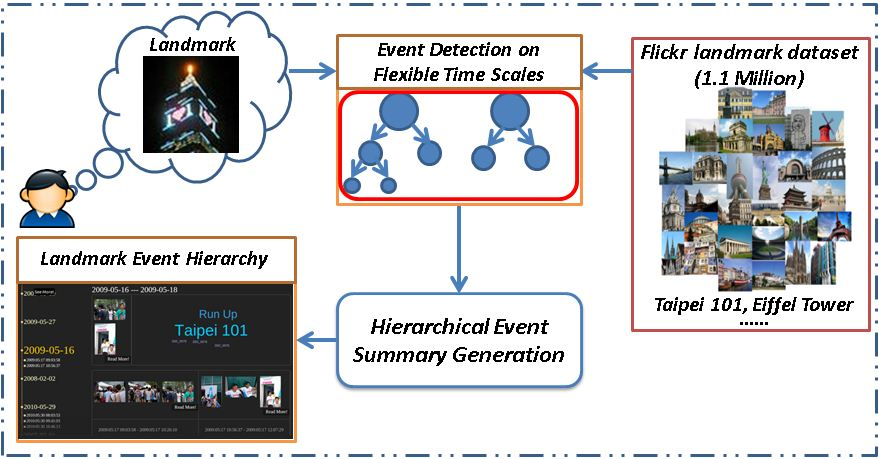
\includegraphics[width=0.9\textwidth]{img/architecture.jpg}
\caption{层次化事件挖掘流程图}
\label{fig:architecture}
\end{figure}

当然,对于视频数据集的事件挖掘也是比较容易的,因为视频本质上就是每秒24张图片,它是一个时间序列的图片数据,本质上来说,
就是时间序列约束下的图片数据集,可以采用我们的方法继续去解决。
更进一步,还可以利用HMM(隐式马尔可夫模型)去构建模型来对相邻时间点的图片关系进行预测。


\section{基于电商平台的衣服搜索}
电子商务越来越成为互联网界最重要的产业,随着阿里巴巴的上市,国内电子商务的力量逐渐被大大的呈现出来。
随之而来的是,中国更多的人拥有了就业机会,中国更多的人通过互联网购买到了最先进最实惠的产品,中国人民的需求被大大的挖掘出来。
服装类商品一直是商业社会中非常重要的产品,在电子商务中,人们一半以上的购物需求基本都是围绕着服装类商品展开。
而现在随着互联网信息的极度膨胀,如果在浩如烟海的电子商务平台上找到自己称心如意的服装,成为一个极大的挑战。
很多时候,我们都觉得上淘宝这样的网站,太过于复杂了。
一想起要搜索一个关键词,然后罗列了100多页的商品供用户选择,用户就会觉得极度的烦恼。本质上一个关键词很难反应用户真实的需求,
因此就会有很多次搜索请求,还很难真正得到用户想要的衣服商品。
如果有基于图片的衣服搜索引擎,那么将会大大减少用户的购买时间。
因为图片比关键词可以表达更丰富的信息,图片中包含了各种各样的显示信息,更容易满足用户的真正需求。
所以,如何去设计一个基于多媒体数据的衣服搜索引擎,就成为如今电子商务平台的一大挑战。

\begin{figure}
\centering
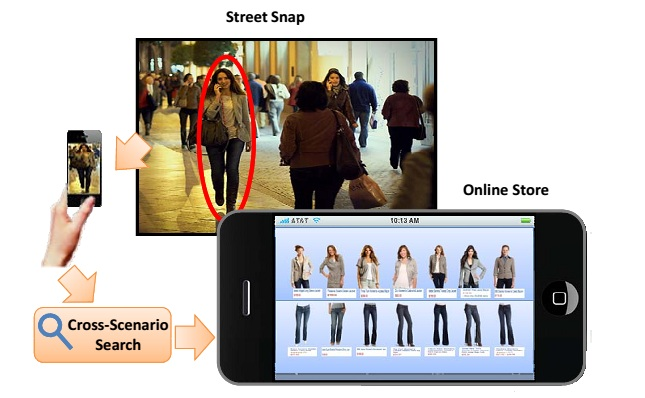
\includegraphics[width=0.9\textwidth]{img/street2shop.jpg}
\caption{衣服搜索模型“Street-to-shop”:用户拍摄一张包含人物的图片后,系统会根据模型算法到电商平台数据库中搜索出最相近的衣服。}
\label{fig:street}
\end{figure}

衣服搜索真正的难题在于,如何从海量衣服数据库中找到和用户输入图片真正匹配的衣服,这往往需要两步进行。
第一步,我们需要分析出用户输入图片中的衣服属性,用这些衣服属性信息去描述这幅图片想要表达的所有关于衣服的语义信息。
第二步,需要设计很好的相似度匹配函数,从而通过输入图片的衣服属性,来寻找最匹配、也就是最满足用户真实需求的衣服。
下面我们就分别详细介绍每一步工作中的难点所在。

\subsection{衣服属性分析}
衣服属性信息是描述图片中衣服最合适的方式,它可以将衣服的信息完整的表达出来,如衣服的袖子长短,衣服的领口样式,衣服的纹理,衣服的品牌,衣服的整体样式等。
如何将这些属性解析出来,是一个难题。我们的方案是首先通过本文中提到的方法去预测人体各个部位的位置和方向,比如手臂的位置、头的位置、躯干的位置等。
当这些人体各个部位的位置都被预测出来后,我们就可以利用这个结果去分析与人体部位相关联的衣服属性。
比如我们知道了手臂的位置,那么就可以检测出衣服的袖子的样式和长短,就得到了袖子这个衣服属性的特征,其它原理是相同的。

\begin{figure}
\centering
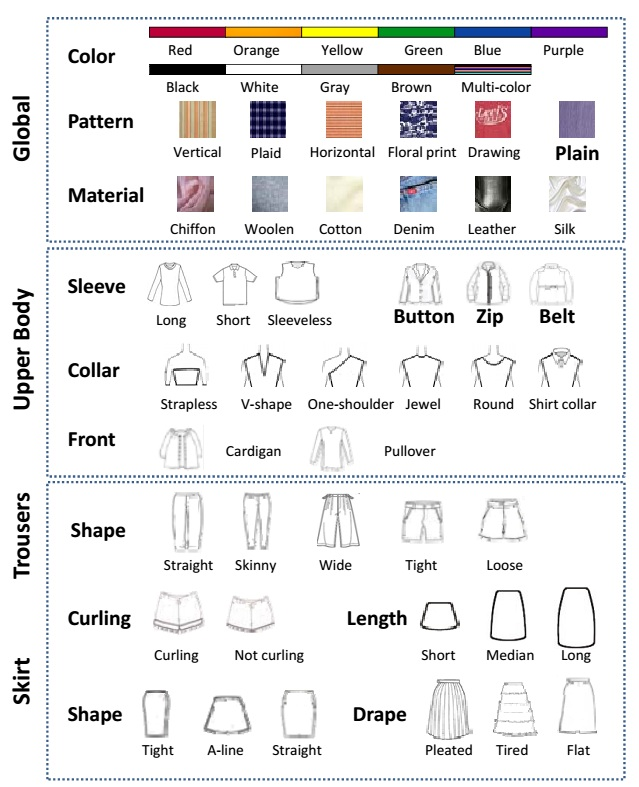
\includegraphics[width=0.9\textwidth]{img/attribute.jpg}
\caption{衣服属性示意图}
\label{fig:attribute}
\end{figure}

\subsection{衣服分类和匹配}
当进行完衣服属性分析后,我们相当于有了一个衣服属性的集合,这个集合里包含了所有的衣服属性(袖子、纹理、衣领等)信息。
首先我们的系统可以根据这些衣服属性对所有的衣服进行分类,每一个衣服属性都可以分很多类,比如袖子这个属性可以分为四类,长袖、中袖、短袖和无袖等。
这样可以为电商平台的服装商品构建一个强大的分类系统,用户根据这个分类系统也可以进行强大的检索行为。
其次,我们需要设计一个强大的、可伸缩的、精准的相似度匹配系统,来通过用户输入图片寻找最合适、最满足用户真实意图的衣服。
一个可行的方案是,将每件衣服都向量化为一个衣服属性特征向量,向量中包含了所有衣服属性信息。
这样我们可以通过标准的向量相似度函数来计算任意两个衣服属性特征向量的相似度。
从而对于用户输入的衣服图片,我们可以选择衣服数据库中相似度最接近的衣服,来推荐给用户。
这样节省了用户大量的时间,来进行搜索购买衣服。

\begin{figure}
\centering
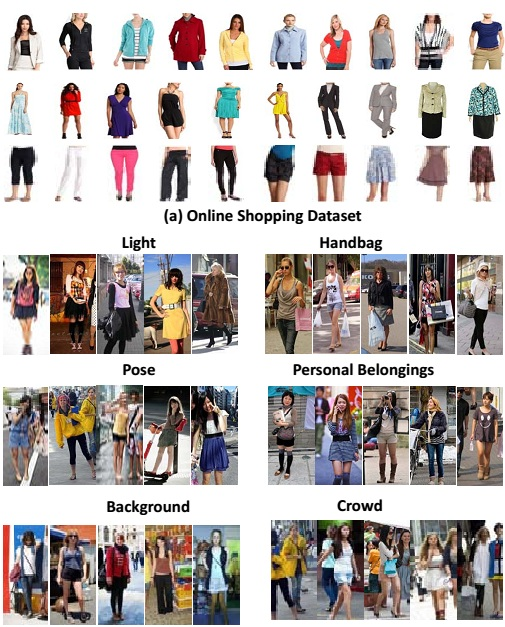
\includegraphics[width=0.9\textwidth]{img/map.jpg}
\caption{衣服属性与衣服匹配图}
\label{fig:attr-cloth}
\end{figure}

\section{基于图片的广告推荐}
广告是互联网时代最伟大的商业模式发明,它为互联网公司找到了流量变现的最强大方式。
从本质上来说,全球基本上所有的互联网公司都是广告公司,基本上百分之八十的收入都来自广告收入。
所以如何提高广告推荐的转化率,是互联网公司都需要面对的问题。
即就是将最精准的广告推送给用户,这个将极大的关乎到互联网公司的营收问题。

%图片

以前是文本广告推荐的模式,如今进入了图片时代,所以基于图片数据如何做广告推荐成为了一个新的挑战。
那我们专注在图片中包含人物的情况下,如何去做广告推荐。
广告是要产生商业价值的东西,所以我们尽可能去挖掘图片上所表达的语义信息,比如人做的动作,在进行斯诺克运动,那么我们可以推荐斯诺克球杆等,
比如人物所穿的衣服,我们可以根据衣服的属性样式去推荐类似的衣服,让用户产生购买的欲望需求。
所以本质上来说,基于图片的广告推荐也就是要去理解图片中表达的语义信息,只有理解了语义信息,才可以针对这些信息去做精准化的广告推荐。


\section{本章小结}
在本章中,我们看到了人体姿势预测任务的一些应用案例,有信息检索领域的、电子商务领域的、广告推荐领域的等。
可以看出,人体姿势预测是计算机视觉领域非常基础的一个问题,解决好了这个问题,那么就可以应用到很多相关领域。
而且我们可以看出,随着互联网的发展,文本数据的方式已经慢慢成熟,而图片时代将慢慢到来,但是文本数据时代积累的经典方法依旧值得我们采纳。
在处理图片数据时,我们还是去理解图片中包含的语义信息,并且可以借鉴文本数据时代的方法。
因此不同数据集上的方法可以是互相借鉴的,只不过处理的方式不同而已。

% experiment
% !Mode:: "TeX:UTF-8"
%%==========================
%% chapter01.tex for SJTU Master Thesis
%% based on CASthesis
%% modified by wei.jianwen@gmail.com
%% version: 0.3a
%% Encoding: UTF-8
%% last update: Dec 5th, 2010
%%==================================================

%\bibliographystyle{sjtu2} %[此处用于每章都生产参考文献]
\chapter{实验结果}
\label{chap:exp}
\section{数据集}
我们在两个数据集上进行了评测,一个是Buffy数据集,一个是DL(daily life)数据集。
Buffy数据集包含了748张从Buffy TV秀中截取下来的图片,每张图片包含了人体各个部位的位置标签。
这个数据集是人体姿势预测问题的标准数据集,很多已有的工作都是在这个上面进行的。
DL数据集包含了997张人体生活照片,是我们从Flickr图片社交分享网站上抓取下来的。
我们对他进行了手工标注,标注了人体各个部位的位置标签。
跟Buffy数据集相比,DL数据集拥有更丰富的衣服属性信息。
为了对我们求解的衣服属性值进行评测,我们手动为Buffy和DL标注了衣服属性标签信息。
为了训练和评测,我们对每个数据集进行了切分。
对于Buffy数据集,选取472张图片作为训练数据集,剩下的作为测试数据集。
对于DL数据集,我们选取200张图片作为训练数据集,剩下的作为测试数据集。

\begin{table}
\centering
\caption{在Buffy数据集上和前人工作的对比}
\begin{tabular}{|c|c|c|c|c|c|} \hline
    Method & Torse & Upper arms & Lower arms & Head & Total \\ \hline
Andriluka et al.~\cite{cvpr09} &  90.7 & 79.3 & 41.2 & 95.5 & 73.5 \\ \hline
Sapp et al.~\cite{eccv10} & \textbf{100} & 95.3 & 63.0 & 96.2 & 85.5 \\ \hline
Yang and Ramanan~\cite{deva11} & \textbf{100} & 96.6 & 70.9 & \textbf{99.6} & 89.1 \\ \hline
Our Approach & \textbf{100} & \textbf{97.1} & \textbf{78.4} & 99.1 & \textbf{91.6} \\ \hline
\end{tabular}
\label{tb:buffy}
\end{table}

\begin{table}
\centering
\caption{在DL数据集上和前人工作的对比}
\begin{tabular}{|c|c|c|c|c|c|} \hline
    Method & Torse & Upper arms & Lower arms & Head & Total \\ \hline
Andriluka et al.~\cite{cvpr09} &  97.0 & 91.7 & 84.5 & 94.0 & 90.6 \\ \hline
Sapp et al.~\cite{eccv10} & \textbf{100} & 88.5 & 78.0 & 87.6 & 86.8 \\ \hline
Yang and Ramanan~\cite{deva11} & 99.8 & 95.7 & 87.5 & 95.6 & 93.6 \\ \hline
Our Approach & \textbf{100} & \textbf{97.2} & \textbf{91.3} & \textbf{99.1} & \textbf{95.7} \\ \hline
\end{tabular}
\label{tb:dl}
\end{table}

\section{实验评测规则}
我们和已有的三份工作进行了对比,包括Andriluka等\cite{cvpr09},Sapp等\cite{eccv10},Yang and Ramanan等\cite{deva11}。
对于人体姿势预测的结果,我们采用标准的评测指标,即就是正确姿势的概率PCP\cite{fer09},它代表了正确的姿势所占的比例。
对于衣服属性的聚类结果,我们采用聚类工作中的标准指标F1分值来进行评测。
我们用$K$-Means聚类的结果作为衣服属性的基准,对于已有的三份工作,我们用他们得到的姿势解来求得最优的衣服属性,然后进行$K$-Means聚类。


\begin{figure}[tbp]
\centering
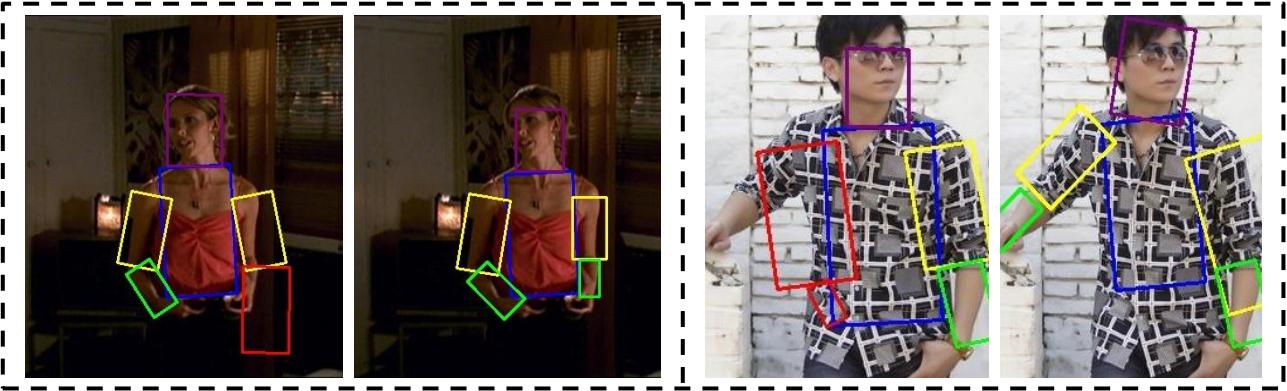
\includegraphics[width=0.9\textwidth]{img/compare.jpg}
\bicaption{\textbf{我们的方法和 Yang and Ramanan~\cite{deva11}的对比 }
第1和3个结果是Yang and Ramanan~\cite{deva11}的方法产生的,我们发现这在上臂和下臂上得到了错误的结果。
而我们的方法(第2和4个)得到了正确的结果。}{\textbf{我们的方法和 Yang and Ramanan~\cite{deva11}的对比 }
第1和3个结果是Yang and Ramanan~\cite{deva11}的方法产生的,我们发现这在上臂和下臂上得到了错误的结果。
而我们的方法(第2和4个)得到了正确的结果。}{Fig}{\textbf{Comparison of our approach with Yang and Ramanan~\cite{deva11} }
Yang and Ramanan~\cite{deva11} produces incorrect estimation (the 1st and 3rd) for upper and lower arms,
while our latent clothing attribute approach produces correct.}
\label{fig:compare}
\end{figure}

\section{实验结果分析}
图6展示了我们算法得出的一些结果,可以定性的看出,我们的算法取得了不错的效果。
在表2和表3中我们分别展示了Buffy和DL数据集的PCP评测结果。
对于Buffy数据集,表2显示我们的方法超越了目前最好的方法Yang and Ramanan\cite{deva11}。
众所周知,下臂的检测是最具有挑战性的,但是令人惊喜的是,我们的方法比目前最好的方法超过了7.5个百分点,这是一个很大的提升了,显示了我们将衣服属性考虑进去的优越性。
对于DL数据集来说,我们的方法超越了目前已有的所有方法。

我们的方法附加的产出是对具有相似衣服属性的图片进行了聚类,图5分别展示了Buffy和DL数据集上的结果。
在图5的上半部分中,我们展示了Buffy数据集的聚类效果,DL数据集的聚类效果在下方。
表4和表5显示了每一种方法的F1分值,可以看出,我们的方法极大的提高了聚类的准确性,比基准要高出很多。
这很大程度上是因为我们的模型训练策略和迭代式的优化算法。
注意到,“$K$-Means+Groundtruth“为我们的模型训练提供了初始的衣服属性标签信息,这也验证了我们方法的有效性。

\begin{table}
\centering
\caption{在Buffy数据集上对衣服属性结果的F1分值}
\begin{tabular}{|c|c|c|c|c|} \hline
    HPE & Sleeve & Neckline & Pattern & Total \\ \hline
Andriluka et al.~\cite{cvpr09} + $K$-Means & 24.1 & 26.6 & 34.2 & 28.3  \\ \hline
Sapp et al.~\cite{eccv10} + $K$-Means & 22.9 & 27.9 & 40.5 & 30.4 \\ \hline
Yang and Ramanan~\cite{deva11} + $K$-Means & 38.3 & 25.7 & 22.6 & 28.9\\ \hline
Groundtruth + $K$-Means & 34.7 & 36.1 & 39.5 & 36.8\\ \hline
Our Approach & \textbf{55.6} & \textbf{68.8} & \textbf{80.8} & \textbf{68.4}  \\ \hline
\end{tabular}
\label{tb:f1_buffy}
\end{table}


\begin{table}
\centering
\caption{在DL数据集上对衣服属性结果的F1分值}
\begin{tabular}{|c|c|c|c|c|} \hline
    HPE & Sleeve & Neckline & Pattern & Total \\ \hline
Andriluka et al.~\cite{cvpr09} + $K$-Means & 27.5 & 31.7 & 27.6 & 28.9  \\ \hline
Sapp et al.~\cite{eccv10} + $K$-Means & 34.9 & 30.5 & 23.8 & 29.7 \\ \hline
Yang and Ramanan~\cite{deva11} + $K$-Means & 43.2 & 28.6 & 35.8 & 35.9 \\ \hline
Groundtruth  + $K$-Means & 31 & 29.8 & 26.1 & 28.9 \\ \hline
Our Approach & \textbf{57.2} & \textbf{60.3} & \textbf{74.7} & \textbf{64.1}  \\ \hline
\end{tabular}
\label{tb:f1_dl}
\end{table}


\begin{figure*}[tbp]
\centering
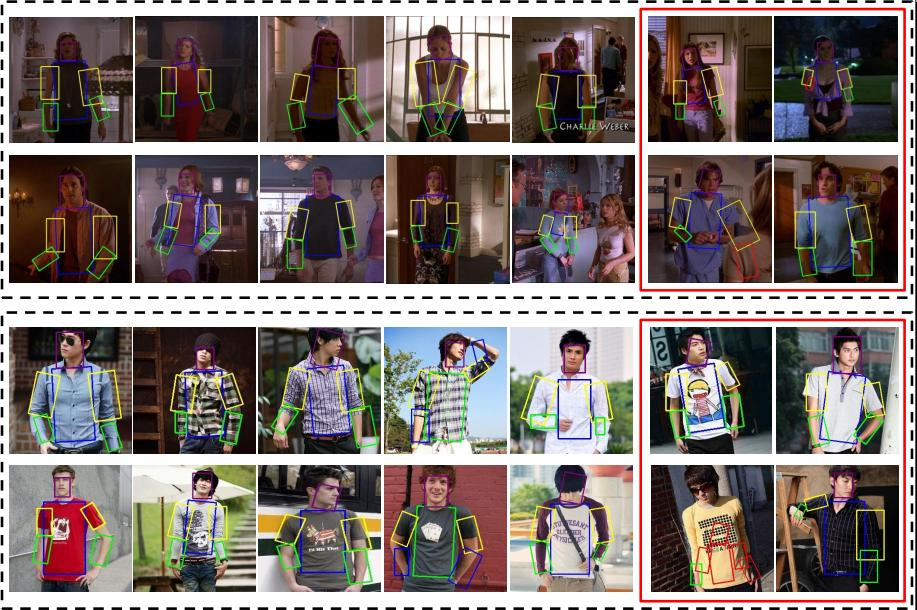
\includegraphics[width=\textwidth]{img/attr.jpg}
\bicaption{\textbf{Buffy上袖子的聚类结果和DL上衣领的聚类结果}
上面的框中的第一行表示袖子类别中的无袖类型,而第二行表示长袖类别。
下面的框中的第一行表示衣领属性中的尖领类别,而第二行代表圆领类别。
这两个框中的第二列都代表每一个属性的错误聚类结果。}{\textbf{Buffy上袖子的聚类结果和DL上衣领的聚类结果}
上面的框中的第一行表示袖子类别中的无袖类型,而第二行表示长袖类别。
下面的框中的第一行表示衣领属性中的尖领类别,而第二行代表圆领类别。
这两个框中的第二列都代表每一个属性的错误聚类结果。}{Fig}{\textbf{Visualization of pose results produced by our algorithm on the Buffy and DL datasets.}
The top two panels are from Buffy and the others are from DL. We use the oriented bounding box to denote the pose estimation.
The first panel of each dataset are correct results, while the second panel are incorrect results.
The bounding box with red color denote the incorrect estimation.}
\label{fig:sleeve}
\end{figure*}

%\section{复杂度分析}

\begin{figure}
\centering
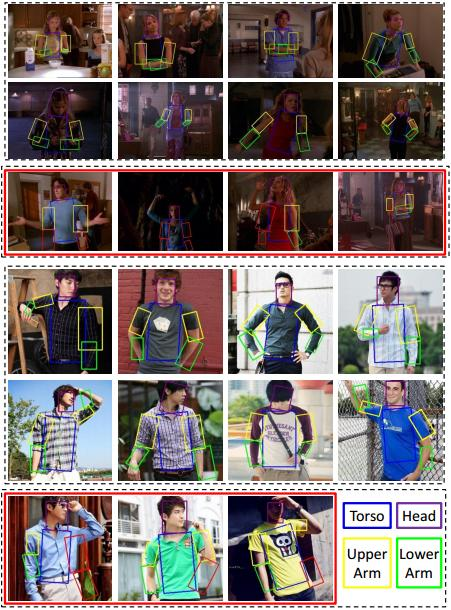
\includegraphics[width=.8\textwidth]{img/result.jpg}
\bicaption{\textbf{我们的算法在Buffy和DL数据集上得到的结果示例}
上面两个框中的结果是Buffy数据集上的,剩下的是DL数据集上的。
我们用带方向的矩形框来表示人体姿势识别的结果。
每个数据集对应的第一个框是正确的结果,而第二个框是错误的结果。
红色的矩形框代表错误的结果,其它颜色分别代表不同的人体躯干部位。}{\textbf{我们的算法在Buffy和DL数据集上得到的结果示例}
上面两个框中的结果是Buffy数据集上的,剩下的是DL数据集上的。
我们用带方向的矩形框来表示人体姿势识别的结果。
每个数据集对应的第一个框是正确的结果,而第二个框是错误的结果。
红色的矩形框代表错误的结果,其它颜色分别代表不同的人体躯干部位。}{Fig}{\textbf{Visualization of pose results produced by our algorithm on the Buffy and DL datasets.}
The top two panels are from Buffy and the others are from DL. We use the oriented bounding box to denote the pose estimation.
The first panel of each dataset are correct results, while the second panel are incorrect results.
The bounding box with red color denote the incorrect estimation.}
\label{fig:result}
\end{figure}

\section{本章小结}
在本章中,我们设计了大量的实验来验证我们提出的方法的可行性,特别是在加进了衣服属性变量以后,
人体姿势预测结果的提升效果。
从定性和定量的角度去对比了我们的工作和前人工作的性能差异,并且分析了我们工作的优势和不足。
同时,我们展示了我们工作的另一个输出结果,将不同照片按照相似的衣服属性聚集在了一起,
这样对于做衣服聚类工作是非常有效的,并且我们利用F1分值对聚类结果进行了评测。
大量实验证明,本文提出的隐变量衣服属性方法取得了目前精度最好的人体姿势预测结果。


% future work & conclusion
% !Mode:: "TeX:UTF-8"
%%==========================
%% chapter01.tex for SJTU Master Thesis
%% based on CASthesis
%% modified by wei.jianwen@gmail.com
%% version: 0.3a
%% Encoding: UTF-8
%% last update: Dec 5th, 2010
%%==================================================

%\bibliographystyle{sjtu2} %[此处用于每章都生产参考文献]
\chapter{总结与展望}
在这篇文章中,我们基于衣服属性和人体姿势之间紧密的联系,提出了将衣服属性作为隐变量,建立人体姿势和衣服属性的联合模型,从而提高人体姿势预测问题的精确度。
相比于前人的一些工作,我们提出的方法不需要进行额外的标注工作,节省了大量的时间,并且可以应用到工业界的大数据中。
对于这个结构化问题,我们采用隐变量结构式支持向量机框架来进行模型参数的学习。
首先,我们采用$K$-Means聚类算法对隐变量进行初始化,然后采用迭代的方式进行模型中人体姿势和衣服属性变量的更新。
由于我们加入了衣服属性变量,原来的图画式无环图问题变成了一个有环图问题,这对于测试图片的最优解预测有着极大的挑战。
我们提出了一个近似迭代算法,用因子图表示问题的结构,采用固定一类变量,然后更新另一类变量的方式求得问题的最优解。
最后,基于两个真实数据集,我们设计了大量实验来验证我们提出的方法。
实验结果表明我们的方法超越了目前最好的结果,并且在时间复杂度上大大降低,高效地解决了人体姿势预测问题。

当然我们的工作中还是有很多可以改进的地方,这也是我们以后的工作方向。
总体来说有以下几个方面:
(1)\textbf{衣服属性的自动挖掘。}衣服属性的定义和选择,是提高人体姿势预测很关键的一个环节。我们目前的思路是选择每个人体躯干对应的衣服属性,
只选择了几种衣服属性,这样肯定是不足的,还有很多很多的衣服属性可以帮助到人体姿势预测,理想的情况是应用到所有的这些信息。
我们希望在以后的工作中,可以提出一种自动挖掘衣服属性的算法,将所有可能帮助到人体姿势预测的衣服属性全部加入到我们的框架当中。
(2)\textbf{特征的自动化学习。}目前我们工作中是人工定义了衣服属性对应的底层图像特征,选择了跟对应的衣服属性最匹配的底层图像特征,
但是也有可能还会有更好的特征或者更好的特征组合。在以后的工作中,我们可以提出一种自动学习出最佳特征或者最佳特征组合的算法,
来为每一个衣服属性选择最佳特征,可能一些Feature Selection(特征选择)的方法有助于这个算法的形成。




%%%%%%%%%%%%%%%%%%%%%%%%%%%%%%
%% 附录(章节编号重新计算,使用字母进行编号)
%%%%%%%%%%%%%%%%%%%%%%%%%%%%%%
\appendix

% 附录中编号形式是"A-1"的样子
\renewcommand\theequation{\Alph{chapter}--\arabic{equation}}
\renewcommand\thefigure{\Alph{chapter}--\arabic{figure}}
\renewcommand\thetable{\Alph{chapter}--\arabic{table}}


%%%%%%%%%%%%%%%%%%%%%%%%%%%%%%
%% 文后(无章节编号)
%%%%%%%%%%%%%%%%%%%%%%%%%%%%%%
\backmatter

%\section{参考文献}
% 使用 BibTeX
% 包含参考文献文件.bib
\bibliography{ref}

%% 个人简历(硕士学位论文没有个人简历要求)
% \include{body/resume}

% 致谢
% !Mode:: "TeX:UTF-8"
%%==========================
%% chapter01.tex for SJTU Master Thesis
%% based on CASthesis
%% modified by wei.jianwen@gmail.com
%% version: 0.3a
%% Encoding: UTF-8
%% last update: Dec 5th, 2010
%%==================================================

%\bibliographystyle{sjtu2} %[此处用于每章都生产参考文献]
\begin{thanks}
在我硕士论文期间,在选题上和论文内容的写作上都得到了俞勇老师精心的指导和建议,而且在硕士学习阶段中,俞老师在生活和学习上对于我都给予了谆谆教导,
特别是在学术交流方面,提倡我们多跟前辈交流,创新都是在思想的激烈碰撞中产生的。
陈佳和沈杰学长在学术小论文方面给予了我大力指导,陈佳学长在我进入研究初期,根据我的特点选择合适的题目,使得我很快进入到研究的领域,并得到了锻炼。
而沈杰学长更是将我带到了一个新的高度,在他严谨的学术态度感染下,我的科研水平得到了迅速提高,特别是在计算机视觉领域,并且发表了国际学术会议论文。
实验室的其它同学也在很多方面帮助了我,特别是潘晔、陈伯良、苏睿龙同学,在学术和生活方面都给了我很大的帮助,并且在课题上进行了大量的交流。
最后,感谢所有实验室帮助过我的同学,没有APEX同学的帮助,我是不可能在学术上走这么长的路。
\end{thanks}


% 发表文章目录
% !Mode:: "TeX:UTF-8"
%%==========================
%% chapter01.tex for SJTU Master Thesis
%% based on CASthesis
%% modified by wei.jianwen@gmail.com
%% version: 0.3a
%% Encoding: UTF-8
%% last update: Dec 5th, 2010
%%==================================================

%\bibliographystyle{sjtu2} %[此处用于每章都生产参考文献]
\begin{publications}{99}

    %\item\textsc{Zhang W, Shen J, Liu G, Yu Y}, et al. {A Latent Clothing Attribute Approach for Human Pose Estimation}[C].
    \item\textsc{1st Author}, et al. {A Latent Clothing Attribute Approach for Human Pose Estimation}[C].
      Proceedings of the 12th Asian conference on Computer Vision. 2014. ACCV'14

    %\item\textsc{Zhang W, Chen J, Shen J, Yu Y}, et al. {Location-Based Hierarchical Event Summary for Social Media Photos}[C].
    \item\textsc{1st Author}, et al. {Location-Based Hierarchical Event Summary for Social Media Photos}[C].
      Proceedings of the 15th Annual Pacific-Rim conference on Multimedia. 2014. PCM'14

    %\item\textsc{Chen J, Jin Q, Zhang W, Bao S, Su Z, Yu Y}, et al. {Tell me what happened here in history}[C].
    \item\textsc{3rd Author}, et al. {Tell me what happened here in history}[C].
      Proceedings of the 21th ACM International conference on Multimedia. 2013. ACM Multimedia'13

\end{publications} 

% 参与项目列表
%\include{body/projects}

\end{document}
